\twocolumn

\chapter{Практическая навигация\label{chap:6}}

Слово <<навигация>> произошло от латинского <<navigatio>> \---
судоходство. Судовождение является предметом штурманской
специальности. От знаний и опыта штурмана зависит безаварийное
плавание судна.

Штурманское дело на яхтах имеет ряд особенностей, осложняющих работу
штурмана. К этим особенностям относятся:
\begin{enumerate}
\item небольшая высота глаза над уровнем моря, что уменьшает видимость
  и усиливает влияние рефракции, искажающей формы предметов;
\item ограниченный обзор, снижающий возможности наблюдения и
  пеленгования;
\item значительные дрейф и рыскливость яхты на волнении и постоянный
  крен, которые вносят ошибки как в счисление, так и в обсервации;
\item обычно слабая оснащённость техническими средствами судовождения. 
\end{enumerate}

\section{Форма и размеры Земли. Географические координаты} 

\begin{figure}[htb]
  \centering{}
  \includegraphics[width=\linewidth]{N001.pdf}
  \caption{Эллипсоид вращения}
  \label{fig:N1}
\end{figure}

В результате исследований установлено, что действительной формой Земли
является геоид \--- неправильное геометрическое тело, близкое по форме
к эллипсоиду вращения (сфероиду). Эллипсоид вращения образуется при
вращении эллипса $P_NQP_SQ'$ вокруг его малой оси $P_NP_S$
(рис.~\ris{N1}). Разность между длинами большой и малой полуосей
земного сфероида составляет только 21\=,382~м, т.\=,е. всего 0,3\,\%
длины большой полуоси. Поэтому при решении большинства навигационных
задач допустимо для упрощения всех расчётов принимать Землю за шар с
радиусом 6\=,371,1~км., имеющий поверхность и объем почти одинаковые с
земным эллипсоидом.

Положение различных объектов на поверхности Земли может быть
определено с помощью географических координат. Для отсчёта координат
на земной шар условно нанесена система точек и кругов (рис.~\ris{N2}).

Введём ряд определений. Воображаемая прямая, вокруг которой происходит
суточное вращение Земли, называется \textbf{земной осью}\index{земная ось}.

Точки пересечения её с поверхностью Земли называются
\index{полюс!географический}\index{полюс!истинный}
\textbf{географическими} или \textbf{истинными полюсами}: северным
$P_N$ и южным $P_S$.

При сечении шара плоскостью получается круг, а на поверхности шара
образуется окружность. Если секущая плоскость проходит через центр
шара, то круг имеет наибольшие размеры и называется
\textbf{большим}. Круги, образующиеся от сечения шара плоскостями, не
проходящими через его центр, называются \textbf{малыми}.

Окружность большого круга $QQ'$, плоскость которого перпендикулярна
земной оси, называется \textbf{экватором}\index{экватор}. Он делит земной шар на
северное и южное полушария.

Окружности малых кругов, плоскости которых параллельны плоскости
экватора, называются \textbf{параллелями}\index{параллели} ($pp'$).

Окружности больших кругов, плоскости которых проходят через ось Земли,
называются \index{меридиан!географический}\index{меридиан!истинный}
\textbf{географическими} или \textbf{истинными
  меридианами}. Половину окружности меридиана $P_NMP_S$, заключённую
между полюсами и проходящую через данную точку $M$, называют
\textbf{меридианом места}\index{меридиан!места}.

Меридиан $P_NGP_S$, проходящий через астрономическую обсерваторию в
Гринвиче (Англия), носит название \textbf{гринвичского}\index{меридиан!гринвичский} (начального)
меридиана. Гринвичский меридиан вместе с противоположным ему
меридианом $P_NG'P_S$ делит земной шар на \textbf{восточное}\index{полушарие!восточное} и
\textbf{западное}\index{полушарие!западное} полушария.

В систему географических координат входят две сферические координаты:
\index{широта}\index{долгота} \textbf{широта} и \textbf{долгота}.

\begin{figure}[htb]
  \centering{}
  \includegraphics[width=\linewidth]{N002.pdf}
  \caption{Географические координаты}
  \label{fig:N2}
\end{figure}

\textbf{Географической широтой}\index{широта!географическая}
какой-либо точки называется угол при центре Земли, составленный
отвесной линией (земным радиусом), проведённой через данную точку, и
плоскостью экватора (угол $MOL$, см. рис.~\ris{N2}). Широта измеряется
дугой меридиана от экватора до параллели данной точки. Она
отсчитывается к северу или югу от экватора от 0 до 90\gr. Если точка
находится в северном полушарии, её широте приписывается наименование
$N$ (северная), если в южном \--- $S$ (южная). Широту обозначают
греческой буквой <<$\varphi$>>.

\textbf{Географической долготой}\index{долгота!географическая}
какой-либо точки называется двугранный угол между плоскостью
гринвичского меридиана и плоскостью меридиана данной точки (угол
$GOL$, см. рис.~\ris{N2}). Долгота измеряется меньшей из дуг экватора
между гринвичским меридианом и меридианом точки и отсчитывается от
гринвичского меридиана к востоку или западу от 0 до 180\gr. Если точка
находится в восточном полушарии, то долготе приписывают наименование
$E$ (восточная), если в западном \--- $W$ (западная). Долготу
обозначают греческой буквой <<$\lambda$>>.

\textbf{Разность широт}\index{широта!разность} и \textbf{разность
  долгот}\index{долгота!разность}. Географические координаты судна в
результате сделанного перехода изменяются. Изменения широты и долготы
судна называются разностями широт и долгот.

\begin{figure*}
  \centering{}
  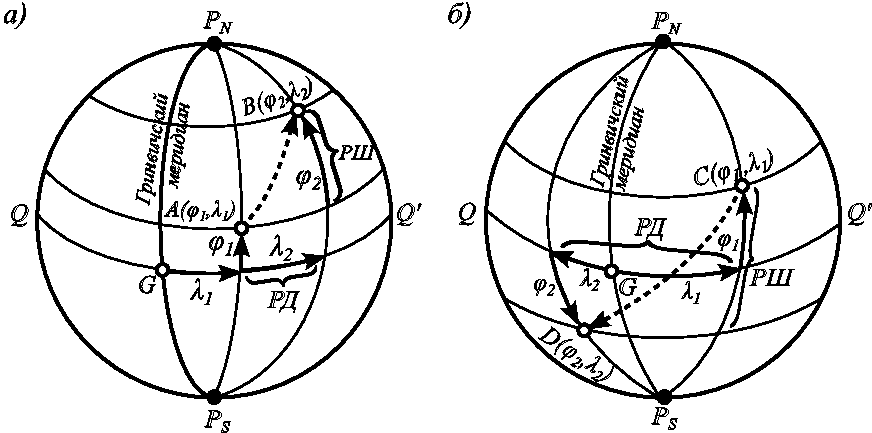
\includegraphics[width=0.8\textwidth]{N003.pdf}
  \caption{Разность широт и разность долгот}
  \label{fig:N3}
\end{figure*}

\textbf{Разность широт} (\textit{РШ}) двух точек на земной поверхности
измеряется дугой меридиана, заключённой между параллелями этих
точек. Наибольшее значение \textit{РШ} может составить 180\gr, что
соответствовало бы перемещению судна из одного полюса в другой. Если
судно перемещалось по какой-либо одной параллели, то \textit{РШ} равна
0\gr. Вычисленной \textit{РШ} приписывается наименование к $N$ или к
$S$ в зависимости от того, в каком направлении перемещалось
судно. Разность долгот (\textit{РД}) двух точек на земной поверхности
измеряется меньшей из дуг экватора, заключённых между меридианами этих
точек. Так как за разность долгот принимается всегда меньшая из дуг
экватора, то её значение не может превышать 180\gr. Если при сложении
разноимённых долгот получено значение, большее 180\gr, то за
\textit{РД} принимается дополнение до 360\gr. Такой случай может
возникнуть при пересечении судном меридиана 180\gr. Вычисленному
значению \textit{РД} приписывается наименование к $E$ или $W$ в
зависимости от того, в каком направлении перемещалось судно. Если
северной широте и восточной долготе условно приписать знак <<плюс>>
($+$), а южной широте знак <<минус>> ($-$), то значение \textit{РШ} и
\textit{РД} можно вычислить по алгебраическим формулам:

\begin{gather}
  \text{\textit{РШ}} = \varphi_2 - \varphi_1\, ; \\
  \text{\textit{РД}} = \lambda_2 - \lambda_1\, ,
\end{gather}

где $\varphi_2$ и $\lambda_2$ \--- координаты конечной, а $\varphi_1$
и $\lambda_1$ \--- начальной точек плавания.

Знак результата, полученного при вычислении по формулам, покажет
наименования \textit{РШ} и \textit{РД}. Если при вычислении
\textit{РД} берётся дополнение до 360\gr, то наименование \textit{РД}
меняется. Чтобы не ошибиться в значении и наименовании вычисляемых
\textit{РШ} и \textit{РД}, следует хорошо представлять взаимное
расположение меридианов и параллелей на земном шаре
(см. рис.~\ris{N3}). На практике бывает нужно найти координаты точки,
в которую пришло судно, если заданы координаты пункта отхода, а также
\textit{РШ} и \textit{РД}, характеризующие положение точки
прихода. Вычисления можно произвести по алгебраическим формулам:

\begin{gather}
  \varphi_2 =  \varphi_1 + \text{\textit{РШ}}\, ; \\
  \lambda_2 =  \lambda_1 + \text{\textit{РД}}\, ,
\end{gather}

где $\varphi_2$ и $\lambda_2$ \--- координаты конечной, а $\varphi_1$
и $\lambda_1$ \--- начальной точек плавания.

\section{Единицы длины и скорости в судовождении}

За основную единицу длины, служащую для измерения расстояний в море, в
судовождении принята морская миля. \textbf{Морской милей}
\index{миля!морская} называется линейное значение $1'$ дуги земного
меридиана. Принято округлённое значение средней величины морской мили,
равное 1852~м. \textit{Кабельтов}\index{кабельтов} \--- единица длины для измерения небольших
расстояний. Он равен одной десятой части мили. Округлённо кабельтов
считается равным 185~м.
 
Глубины моря и высоты предметов на большинстве навигационных карт
измеряются в метрах. На старых английских картах для указания высот
предметов применялись футы (0,3048~м), а для указания глубин \--- футы
и морские сажени (6~футов, или 1,83~м). Скорость судна при плавании в
море измеряют узлами.

Узел \--- это единица скорости, равная 1 морской миле в час,
т.\=,е. 1,852~км/ч.

\section{Основные линии и плоскости наблюдателя}

Для ориентирования в море принята система условных линий и плоскостей
наблюдателя.

На рис.~\ris{N4} изображён земной шар, на поверхности которого в точке
$M$ располагается наблюдатель.

Его глаз находится в точке $A$. Буквой $e$ обозначена высота глаза
наблюдателя над уровнем моря.

\begin{figure}[htb]
  \centering{}
  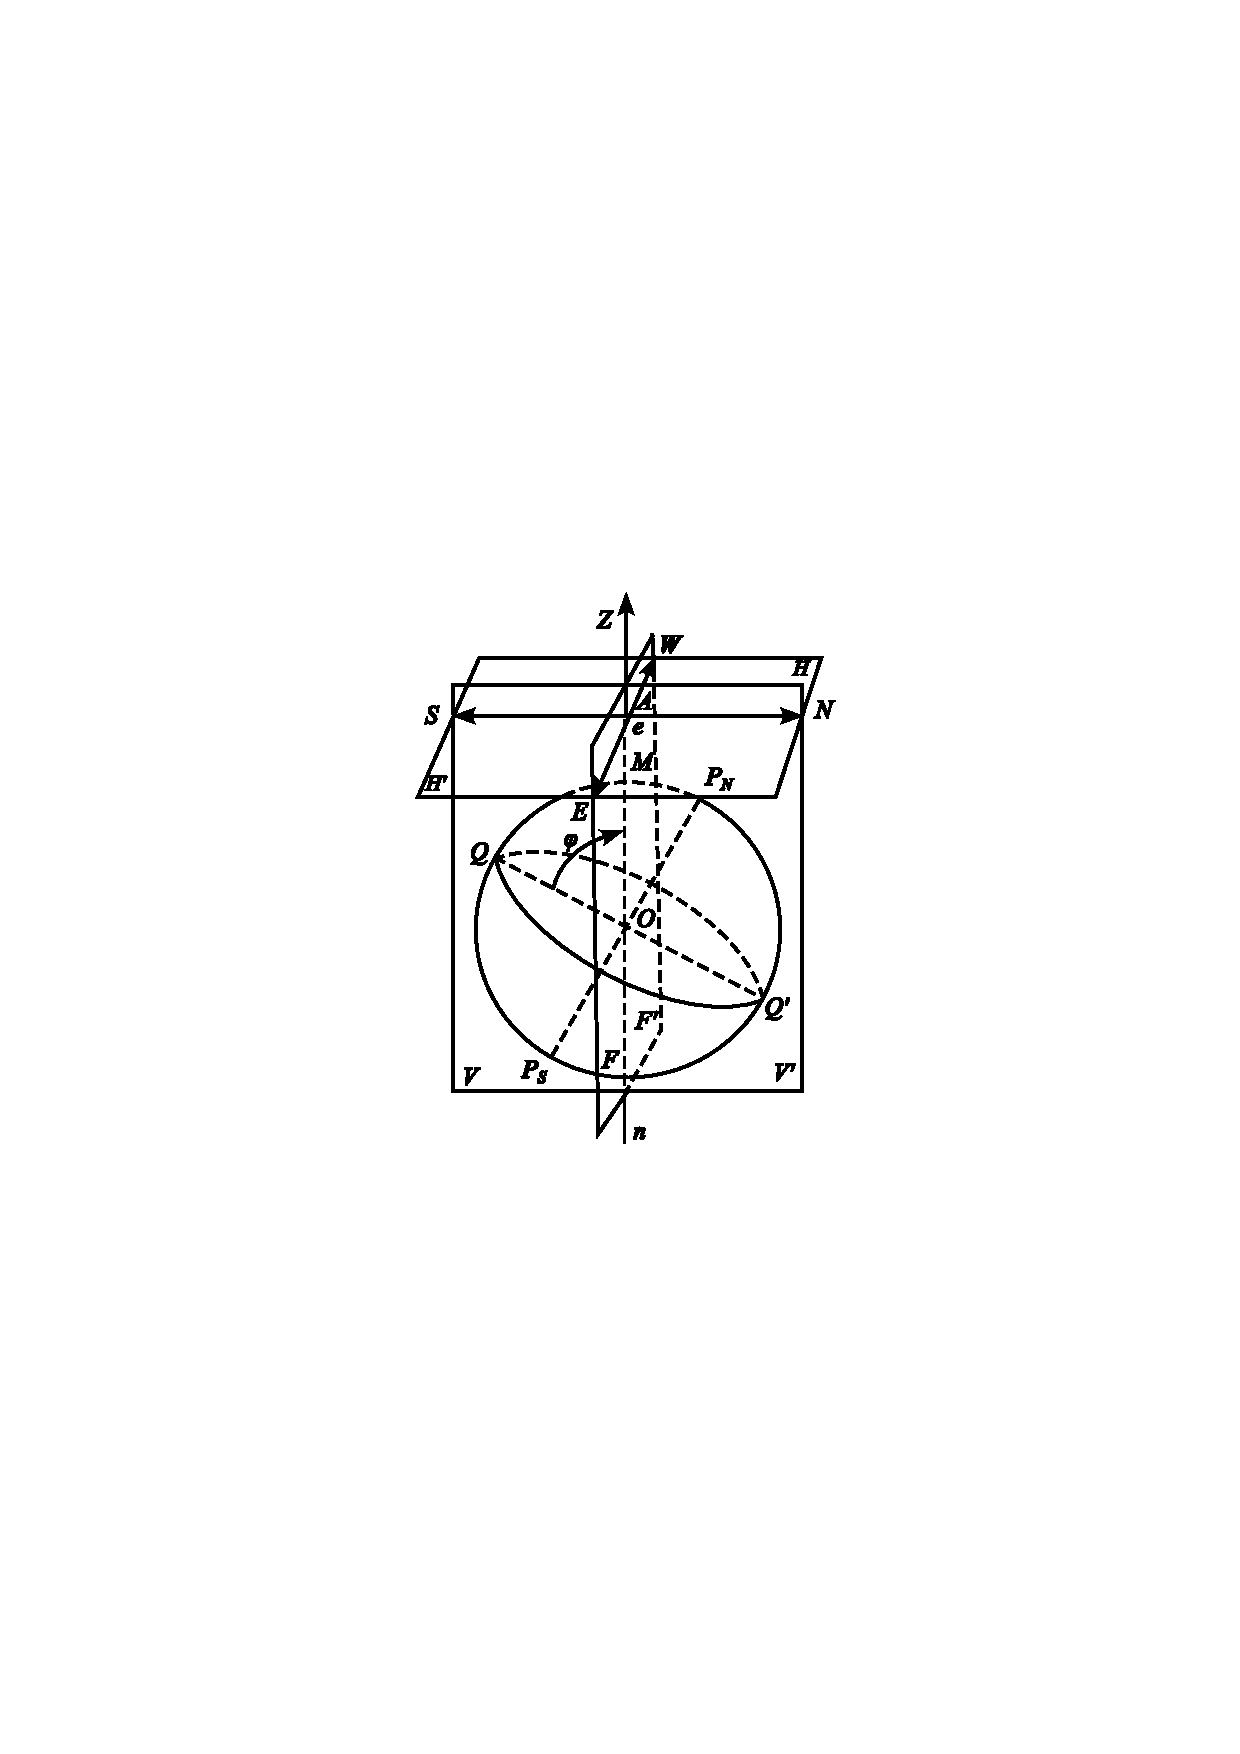
\includegraphics[width=\linewidth]{N004.pdf}
  \caption{Основные линии и плоскости наблюдателя}
  \label{fig:N4}
\end{figure}

Линия $ZMn$, проведённая через место наблюдателя и центр земного шара,
называется \textit{отвесной или вертикальной линией}. Все плоскости,
проведённые через эту линию, называются вертикальными, а
перпендикулярные ей \--- горизонтальными.

Горизонтальная плоскость $HH'$, проходящая через глаз наблюдателя,
называется \textit{плоскостью истинного горизонта наблюдателя}.

Вертикальная плоскость $VV'$, проходящая через место наблюдателя $M$ и
земную ось, называется \textit{плоскостью истинного меридиана}.

В пересечении этой плоскости с поверхностью Земли образуется большой
круг $P_NQP_SQ'$, называемый \textit{истинным меридианом наблюдателя}.

Прямая, полученная от пересечения плоскости истинного горизонта с
плоскостью истинного меридиана, называется \textit{линией истинного меридиана
или полуденной линией} $N-S$. Этой линией определяется направление на
северную и южную точки горизонта.

Вертикальная плоскость $FF'$, перпендикулярная плоскости истинного
меридиана, называется \textit{плоскостью первого вертикала}. В пересечении с
плоскостью истинного горизонта она образует линию $E-W$,
перпендикулярную линии $N-S$ и определяющую направления на восточную и
западную точки горизонта.

Линии $N-S$ и $E-W$ делят плоскость истинного горизонта на четверти:
$NE$, $SE$, $SW$ и $NW$.

Плоскость истинного горизонта наблюдателя $HH'$ может быть
представлена только в воображении.

\section{Видимый горизонт наблюдателя и его дальность}

В открытом море наблюдатель видит вокруг судна водную поверхность,
ограниченную малым кругом $CC_1$ (рис.~\ris{N5}). Этот круг называется
\textit{видимым горизонтом наблюдателя}.

Расстояние $D_e$ от места судна $M$ до линии видимого горизонта $CC_1$
называется дальностью видимого горизонта.

\begin{figure}[htb]
  \centering{}
  \includegraphics[width=\linewidth]{N005.pdf}
  \caption{Видимый горизонт наблюдателя}
  \label{fig:N5}
\end{figure}

Теоретическая дальность видимого горизонта $D_T$ (отрезок $AB$) всегда
меньше его действительной дальности $D_e$. Это объясняется тем, что
из-за различной плотности слоев атмосферы по высоте луч света
распространяется в ней не прямолинейно, а по кривой $AC$. В результате
наблюдатель может видеть дополнительно некоторую часть водной
поверхности, расположенную за линией теоретического видимого горизонта
и ограниченную малым кругом $CC_1$. Этот круг и является \textit{линией
видимого горизонта наблюдателя}.

Явление преломления световых лучей в атмосфере называется
\textit{земной рефракцией}\index{земная рефракция}. Рефракция зависит
от атмосферного давления, температуры и влажности воздуха\index{влажность воздуха}. В одном и
том же месте Земли рефракция может меняться даже на протяжении одних
суток. Поэтому при расчётах берут среднее значение рефракции. Формула
для определения дальности видимого горизонта:
%
\begin{equation}
  D_e = 2,08 \sqrt{e} \, ,
\end{equation}
%
где $D_e$ в морских милях; $e$ \--- высота глаза наблюдателя над
уровнем моря \--- в метрах.

В результате рефракции наблюдатель видит линию горизонта в направлении
$AC'$ (см. рис.~\ris{N5}), касательном к дуге $AC$. Эта линия
приподнята на угол $r$ над прямым лучом $AB$. Угол $r$ также
называется земной рефракцией. Угол $d$ между плоскостью истинного
горизонта $HH'$ и направлением на видимый горизонт называется
\textbf{наклонением видимого горизонта}.

\section{Дальность видимости предметов и огней}

Дальность видимого горизонта позволяет судить о видимости предметов,
находящихся на уровне воды. Если предмет имеет определённую высоту $h$
над уровнем моря, то наблюдатель может обнаружить его на расстоянии:
%
\begin{equation}
  D_N = D_h + D_e = 2,08 \sqrt{e} + 2,08 \sqrt{h} \, , 
\end{equation}
%
где: $D_N$ в морских милях, $e$ \--- высота глаза наблюдателя над
уровнем моря \--- в метрах, $h$ \--- высота предмета над уровнем моря
\--- в метрах.

\begin{figure*}[htb]
  \centering{}
  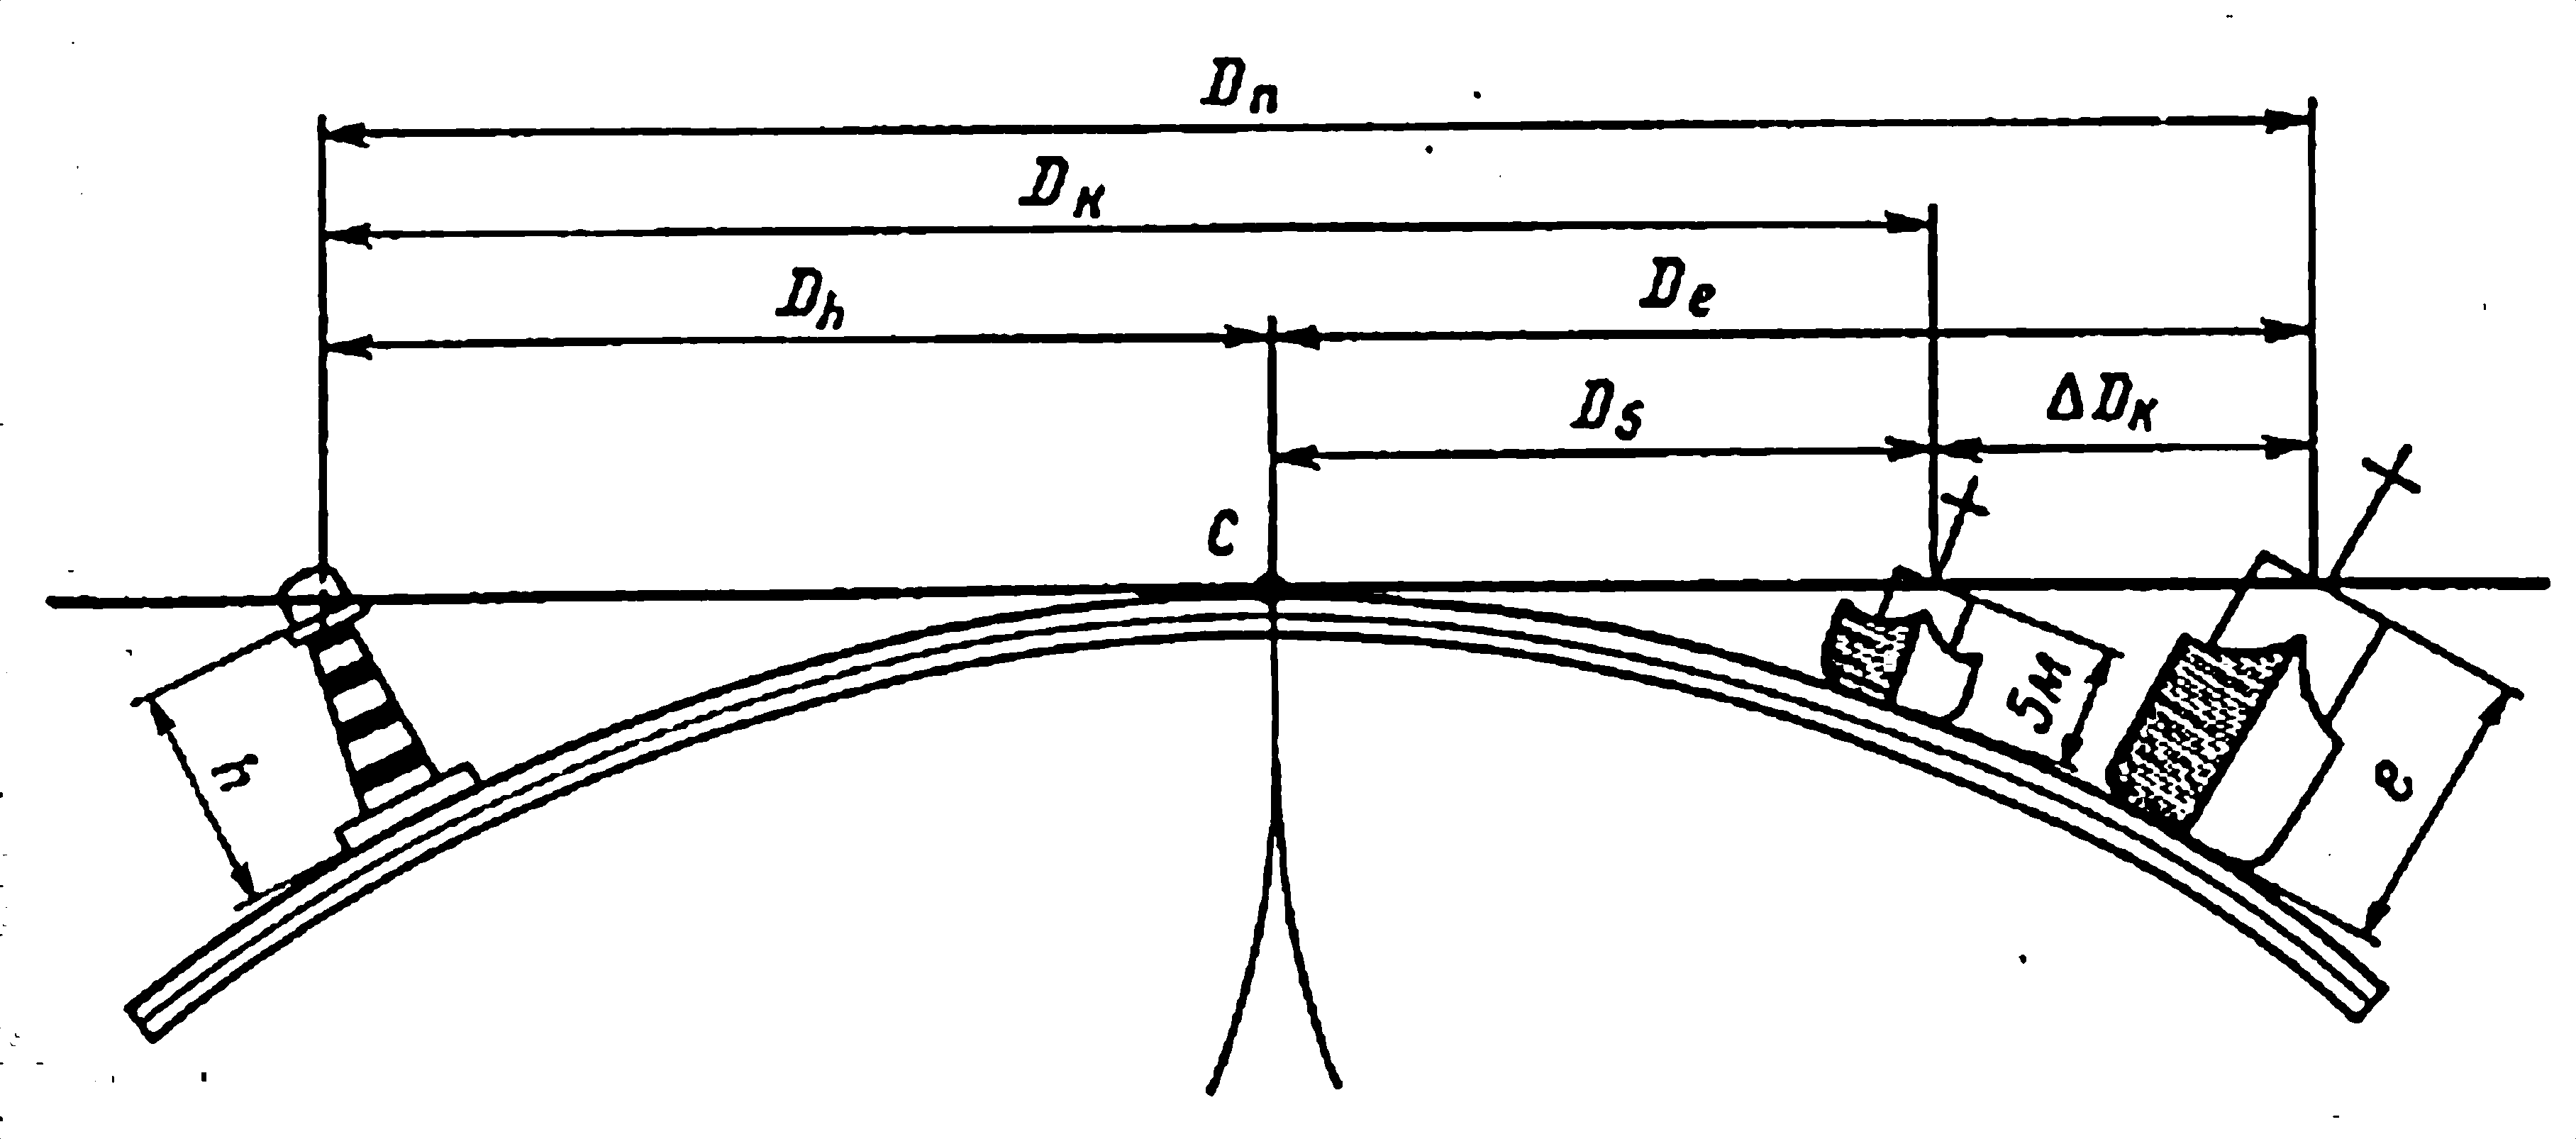
\includegraphics[width=0.8\textwidth]{N006.png}
  \caption{Дальность видимости предмета}
  \label{fig:N6}
\end{figure*}

На морских картах и в навигационных пособиях приводится заранее
вычисленная дальность видимости огней маяков $D_K$ с высоты глаза
наблюдателя 5~м. С такой высоты $D_e$ равна 4,7 мили. При $e$,
отличной от 5~м, следует вносить поправку. Её величина равна:

\begin{equation}
  \Delta D_K = 2,08 \sqrt{e} - 4,7 
\end{equation}

Тогда дальность видимости маяка $D_n$ равна: 
%
\begin{equation}
  D_n = D_K +  \Delta D_K 
\end{equation}
%
где: $D_n$, $D_K$ и $D_K$ в морских милях, $e$ \--- высота глаза
наблюдателя над уровнем моря \--- в метрах.
 
Дальность видимости предметов, рассчитанная по данной формуле,
называется геометрической, или географической. Вычисленные результаты
соответствуют некоторому среднему состоянию атмосферы в дневное время
суток. При мгле, дожде, снегопаде или туманной погоде видимость
предметов, естественно, сокращается. Наоборот, при определённом
состоянии атмосферы рефракция может быть очень большой, вследствие
чего дальность видимости предметов оказывается значительно больше
рассчитанной.

\section{Системы деления горизонта}

\begin{figure}[htb]
  \centering{}
  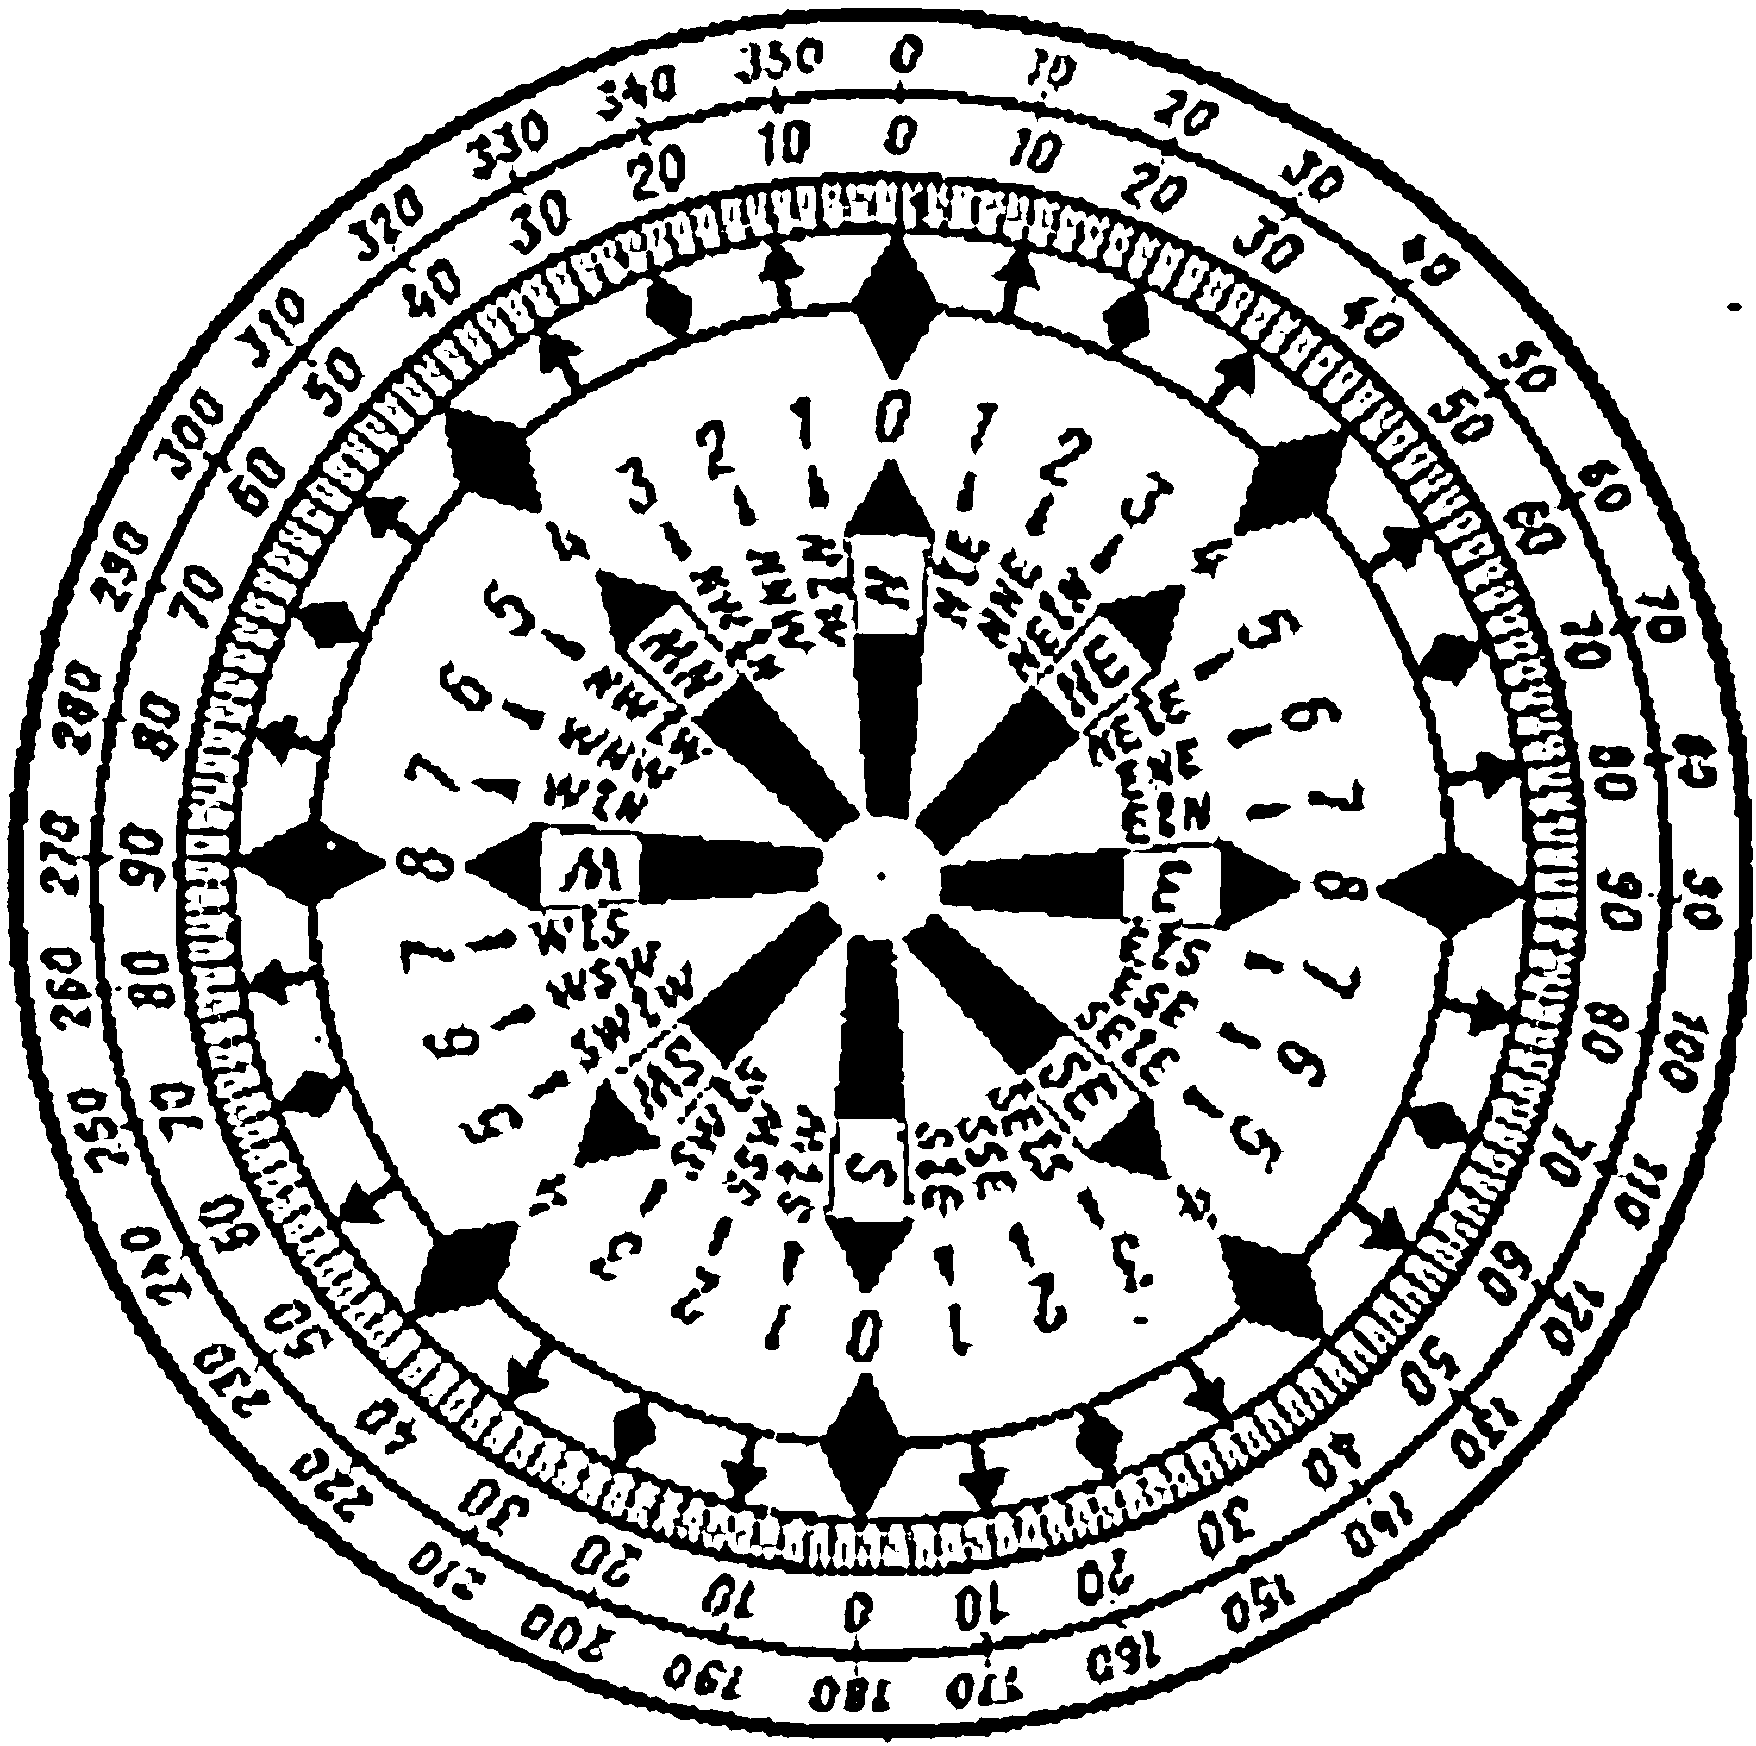
\includegraphics[width=\linewidth]{N007.png}
  \caption{Системы деления горизонта}
  \label{fig:N7}
  \small
  \centering{}
  внутренний круг \--- румбовая; средний \--- четвертная; наружный \--- круговая
\end{figure}

Направления на поверхности Земли наиболее удобно определять путём
измерения горизонтальных углов между плоскостью истинного меридиана
наблюдателя и вертикальной плоскостью, проведённой, например, через
тот или иной ориентир или совпадающей с диаметральной плоскостью
судна.

В эпоху парусного флота направления в море указывались в румбах
(направлениях). По этой системе весь горизонт делится на 32 румба, из
которых четыре отнесены к главным ($N$, $E$, $S$ и $W$), четыре \--- к
четвертным ($NE$, $SE$, $SW$ и $NW$), восемь, расположенных между
главными и четвертными румбами \--- к трёхбуквенным ($NNE$, $ENE$,
$ESE$ и т.\=,д.) и ещё шестнадцать \--- к промежуточным румбам
(рис.~\ris{N7}). Название трёхбуквенных румбов складывается из
названий главных и четвертных, между которыми они находятся. Название
промежуточных румбов состоит из названия ближайшего главного или
четвертного румба, приставки <<тэн>> (ten), которая означает предлог
<<к>>, и названия главного румба, в сторону которого уклонён данный
промежуточный румб. Угол в 11\gr 1/4 между двумя смежными румбами
также называется румбом. В каждой четверти горизонта румбы имеют
порядковые номера от 1 до 8, причём нумерация румбов ведётся от $N$
или $S$ в обе стороны: к $E$ и $W$.

С появлением судов с механическими двигателями и повышением точности
судовождения истинный горизонт стали делить на 360\gr, а счёт
направлений в румбах применять лишь для указания направления ветров,
волнения и течения. Первоначально была введена четвертная система
деления горизонта на градусы. За начало отсчёта в ней принимаются два
направления \--- $N$ и $S$, от которых счёт ведётся к $E$ или $W$ от О
до 90\gr. В настоящее время в навигации принято отсчитывать
направления только от $N$-й части истинного меридиана по часовой
стрелке от 0 до 360\gr. Такая система деления истинного горизонта
носит название круговой (см. рис.~\ris{N7}).

\section{Истинные курсы и пеленги. Курсовой угол} 

\textbf{Путевым углом}\index{путевой угол} называют двугранный угол
между нордовой частью плоскости истинного меридиана и вертикальной
плоскостью, совпадающей с линией перемещения судна.

\begin{figure}[htb]
  \centering{}
  \includegraphics[width=\linewidth]{N008.pdf} % was N008 
  \caption{Изображение истинного курса, истинного пеленга и курсового угла}
  \label{fig:N8}
\end{figure}

Если на судно не влияет ветер, вызывающий дрейф и течение, линия
перемещения судна совпадает с направлением его диаметральной
плоскости. В этом случае направление движения судна определяется
истинным курсом. \textbf{Истинным курсом}\index{курс!истинный} (\IK) называется двугранный
угол между нордовой частью плоскости истинного меридиана и носовой
частью диаметральной плоскости судна.

Направление на ориентир определяется двугранным углом между нордовой
частью плоскости истинного меридиана и вертикальной плоскостью,
проходящей через место наблюдателя и ориентир. Этот угол называется
\textbf{истинным пеленгом}\index{пеленг!истинный} (\IP). Оба угла отсчитываются от нордовой
части истинного меридиана по часовой стрелке от 0 до 360\gr. Угол,
отличающийся от \IP на 180\gr, называется
\textbf{обратным истинным пеленгом}\index{пеленг!обратный истинный} (\OIP):

\begin{gather}
  \IP = \IK + \KU \\
  \IK = \IP - \KU \\
  \KU = \IP - \IK
\end{gather}

Если \KU задан по полукруговому счету, то \IP и \IK вычисляют по формулам: 

\begin{gather}
  \IP = \IK + \Kpb \text{\ или} \\ \IP = \IK - \Klb \\
  \IK = \IP - \Kpb \text{\ или} \\ \IK = \IP + \Klb 
\end{gather}

Когда \KU предмета равен 90\gr правого или левого борта, то говорят,
что предмет находится на \textit{траверзе}\index{траверза}, указывая
при этом наименование борта.

\section{Земной магнетизм. Магнитное склонение. Магнитные курсы и пеленги} 

\begin{figure}[htb]
  \centering{}
  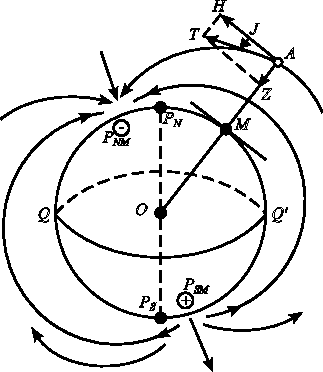
\includegraphics[width=\linewidth]{N009.pdf}
  \caption{Магнитное поле Земли}
  \label{fig:N9}
\end{figure}

В магнитном отношении Земля представляет собой огромный по величине
магнит, магнитное поле которого окружает земной шар. Магнитные полюсы
Земли располагаются сравнительно недалеко от географических, но с ними
не совпадают. Кроме того, они постепенно изменяют своё положение.

Силовые линии магнитного полюса Земли выходят из южного магнитного
полюса $P_S$ и замыкаются в северном $P_N$ (рис.~\ris{N9}).

Магнитное поле Земли в каждой его точке характеризуется величиной его
\textbf{напряжённости $T$}, т.\,е силой, которая действует на единицу
положительного магнетизма, и направлением этой силы. Вектор \ve{T}
направлен по касательной к силовой линии. Разложив полную напряжённость
магнитного поля Земли на горизонтальную $H$ и вертикальную $Z$ составляющие,
заметим, что горизонтальная составляющая удерживает магнитную стрелку,
помещённую в поле Земли, в направлении магнитной силовой линии, а вертикальная
\--- наклоняет стрелку.

Вертикальный угол между осью свободно подвешенной магнитной стрелки
и горизонтальной плоскостью называется \textbf{магнитным наклонением $I$}.
На магнитных полюсах наклонение максимальное и равно 90\gr.
По мере удаления от полюсов оно уменьшается, По мере удаления от
полюсов оно уменьшается пока не достигнет 0\gr.

Кривые, соединяющие по земной поверхности точки с одинаковым магнитным
наклонения называются \textbf{изоклинами}. Нулевая изоклина вдоль которой
наклонение равно 0\gr называется \textbf{магнитным экватором}.

Между составляющими земного магнетизма и магнитным наклонением существует зависимость:

\begin{equation}
  \label{eq:30}
  \begin{split}
      H = T \cos I,\\
    Z = T \sin I.
  \end{split}
\end{equation}

Горизонтальная составляющая $H$ устанавливает магнитную стрелку в
плоскости магнитного меридиана и удерживает её в этом положении. Из
формулы (\ref{eq:30}) следует, что на магнитном экваторе, где
$I=0\gr$, горизонтальная составляющая имеет максимальную величину,
т.\,е. $H=T$, а вертикальная $Z=0$. Поэтому магнитный компас лучше
работает вблизи магнитного экватора и не работает в районе магнитных
полюсов.

Вертикальная плоскость, проходящая через ось свободно подвешенной
магнитной стрелки, называется \textbf{плоскостью магнитного меридиана}, а след
от пересечения этой плоскости с плоскостью истинного горизонта \---
\textbf{магнитным меридианом} $N_M - S_M$ (рис.~\ris{N10}).

Горизонтальный угол, на который в данной точке Земли плоскость
магнитного меридиана отклоняется от плоскости истинного меридиана,
называется \textit{магнитным склонением}\index{склонение!магнитное}
$d$. Оно отсчитывается от северной части истинного меридиана $N_M$ к
$E$ или к $W$ от 0 до 180\gr. Если северная часть магнитного меридиана
$N_M$ отклонена от $N_M$ к востоку, то склонение имеет наименование
$E$ (восточное) и ему приписывается знак плюс ($+$), если к западу, то
$W$ (западное) со знаком минус ($-$).

\begin{figure}[htb]
  \centering{}
  \includegraphics[width=\linewidth]{N010.pdf}
  \caption{Магнитное склонение}
  \label{fig:N10}
  \small
  \centering{}
  $d_E$ \--- восточное; $d_W$ \--- западное
\end{figure}

В отдельных точках Земли магнитное склонение отличается как по
значению, так и по наименованию. В большей части судоходных районов
склонение не превышает 25\gr $E$ или $W$. Исключением являются высокие
широты, где склонение может достигнуть десятков градусов, а между
одноимёнными магнитными и географическими полюсами даже 180\gr.

Кривые линии, соединяющие на картах точки с одинаковым склонением,
называются \textbf{изогонами}, а с нулевым склонением \--- \textbf{агонами}.

Величины $T$, $H$, $Z$, $I$, $d$ называются элементами земного магнетизма,
из них важнейшим для навигации является \textbf{магнитное склонение $d$}.

Чтобы правильно использовать магнитный компас, необходимо знать
значение магнитного склонения в районе плавания. С этой целью на
навигационные карты наносят значение и наименование склонения. Однако
наблюдениями установлено, что значение склонения не остаётся
постоянным даже в одном и том же месте. В отдельных районах за год
склонение может изменяться до 0,2\otdo 0,3\gr. Поэтому на
навигационных картах указывают также год, к которому отнесено
склонение, и значение его годового изменения. Эти сведения наносят
различными способами. Обычно надписи о значении склонения помещают в
центре картушек, размещённых на водной поверхности. Иногда такие же
надписи наносят на карту без изображения картушек, например
<<Магн. скл. 1,2\gr $W$>>. Если значение склонения одинаково для всего
района, охватываемого картой, то данные о нем помещают в заголовке
карты. Значение годового изменения склонения обычно указывают в
заголовке карты, однако, если оно неодинаково в разных районах карты,
его показывают рядом со сведениями о значении склонения.

Магнитное склонение, учитываемое при расчёте поправки компаса,
необходимо приводить к году плавания. Для этого к нанесённому на карте
склонению прибавляют или вычитают из него годовое изменение склонения,
умноженное на разность лет между годом фактического плавания и годом,
к которому относится склонение на карте. Приведённые склонения при
подготовке карт к предстоящему плаванию записывают простым карандашом
рядом со старыми, которые зачёркивают. Если место судна находится в
районе, расположенном между двумя обозначениями склонения, то нужное
склонение определяют путём интерполяции.

В наиболее изученных морях магнитное склонение известно с точностью до
$\pm 0,5\gr$. В океанах, менее изученных в магнитном отношении, ошибки
в выбранных значениях склонения могут достигать $\pm 1\motdo 2\gr$. В
некоторых пунктах земной поверхности склонение резко отличается от его
среднего значения для данного района моря или океана. Такое явление
носит название магнитной аномалии. \textbf{Магнитные
  аномалии}\index{аномалии!магнитные} возникают в местах, где под
поверхностью Земли имеется скопление магнитных пород, создающих
добавочное магнитное поле. Границы аномалий очерчены на морских картах
кривыми чёрными линиями с указанием крайних пределов изменения
магнитного склонения. При плавании в таких районах показания
магнитного компаса ненадёжны. Протекающие на Солнце явления могут
вызывать внезапные и резкие изменения склонения и других элементов
земного магнетизма. Продолжительность таких изменений составляет от
нескольких часов до нескольких суток, их называют магнитными
бурями. Во время магнитных бурь показания магнитных компасов
ненадёжны.

\begin{figure*}
  \centering{}
  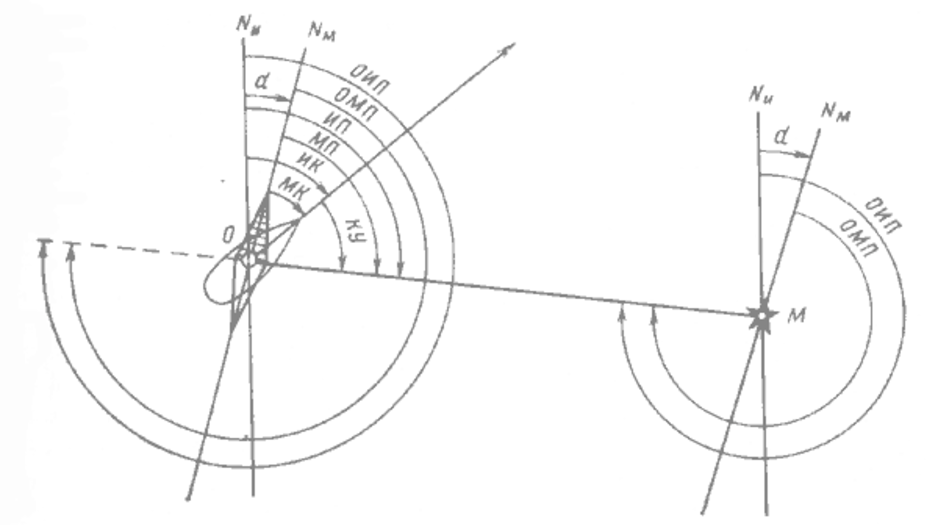
\includegraphics[width=0.8\textwidth]{N011.pdf}
  \caption{Зависимость между истинными и магнитными направлениями}
  \label{fig:N11}
\end{figure*}

Магнитным курсом называется угол в плоскости истинного горизонта,
отсчитываемый от нордовой части магнитного меридиана по часовой
стрелке до носовой части диаметральной плоскости судна; магнитным
пеленгом называется угол в плоскости истинного горизонта,
отсчитываемый от нордовой части магнитного меридиана по часовой
стрелке до направления на ориентир (рис.~\ris{N11}). Угол, отличающийся
от \MP на 180\gr, называется \textit{обратным магнитным
  пеленгом}\index{пеленг!обратный магнитный} (\OMP):
$\OMP = \MP \pm 180\gr$ или $\MP = \OMP \pm 180\gr$. Магнитные курсы и
пеленги могут лежать в пределах от 0 до 360\gr. Зная магнитное
склонение в данном месте Земли, можно по известным магнитным
направлениям получить истинные, а также решить обратную
задачу. Зависимость между магнитными и истинными направлениями
выражается формулами:

\begin{gather}
  \IK = \MK + d \\
  \IP = \MP + d \\
  \OIP = \OMP + d 
\end{gather}

\begin{gather}
  \MK = \IK - d \\
  \MP = \IP - d \\
  \OMP = \OIP - d 
\end{gather}

Формулы алгебраические. Представляемое в них берётся со знаком плюс
($+$) $E$ или минус ($-$) $W$.

\section{Девиация магнитного компаса. Компасные курсы и пеленги} 

Находящиеся в магнитном поле Земли детали набора и другие стальные и
железные части судна постепенно намагничиваются и приобретают свойства
магнита. В результате этого в окружающем судно пространстве возникает
собственное магнитное поле, действие которого складывается с магнитным
полем Земли. Магнитная стрелка судового компаса устанавливается по
равнодействующей сил обоих полей, вследствие чего отклоняется от
направления магнитного меридиана. Горизонтальный угол, на который
плоскость компасного меридиана отклоняется от плоскости магнитного
меридиана, называется \textit{девиацией магнитного
  компаса}\index{девиация} <<$\delta$>> (рис.~\ris{N12}). Девиация
отсчитывается от северной части магнитного меридиана $N_K$ к $E$
(соответственно, со знаком $+$) или $W$ (со знаком $-$) от 0 до
180\gr.

\begin{figure}[htb]
  \centering{}
  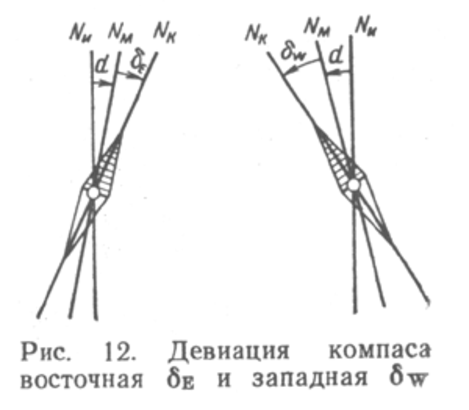
\includegraphics[width=\linewidth]{N012}
  \caption{Девиация компаса}
  \label{fig:N12}
  \small
  \centering{}
  $\delta_E$ \--- восточная; $\delta_W$ \--- западная
\end{figure}

\begin{figure*}[htb]
  \centering{}
  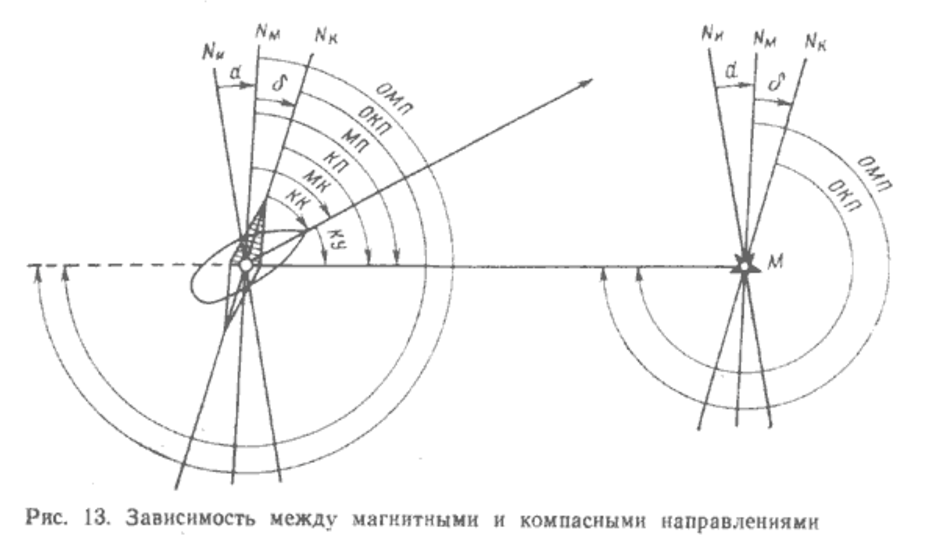
\includegraphics[width=0.8\linewidth]{N013}
  \caption{Зависимость между магнитными и компасными направлениями}
  \label{fig:N13}
\end{figure*}

На каждом курсе девиация у судовых компасов различна. Это объясняется
тем, что при изменении курса меняется положение судового железа
относительно магнитных стрелок компаса. Кроме того, после поворота
судна судовое железо частично перемагничивается, что также приводит к
изменению магнитного поля судна. Девиация судовых компасов изменяется
на одном и том же курсе при перемене широты места, что связано с
изменением напряжённости магнитного поля Земли и, следовательно,
изменением намагниченности судового железа, а также при каждой
погрузке или выгрузке грузов, обладающих магнитными свойствами, при
длительной стоянке судна в ремонте, при проведении электросварочных
работ вблизи компасов, при сильном сотрясении металлического корпуса
судна.

Девиацию судового компаса периодически определяют для различных курсов
и заносят в специальную \textit{таблицу}\index{девиация!таблица},
откуда её выбирают при расчётах курсов и пеленгов. Зная значение
девиации, можно по замеченным компасным направлениям рассчитывать
направления относительно магнитного меридиана. \textit{Компасным
  курсом}\index{курс!компасный} (\KK) называется угол в плоскости
истинного горизонта, отсчитываемый от нордовой части компасного
меридиана по часовой стрелке до носовой части диаметральной плоскости
судна; \textit{компасным пеленгом}\index{пеленг!компасный} (\KP)
называется угол в плоскости истинного горизонта, отсчитываемый от
нордовой части компасного меридиана по часовой стрелке до направления
на ориентир. Угол, отличающийся от \KP на 180\gr, называется \textit{обратным
компасным пеленгом}\index{пеленг!обратный компасным} \OKP:

\begin{gather}
  \OKP = \KP \pm 180\gr \text{\ или} \\
  \KP = \OKP \pm 180\gr
\end{gather} 

Компасные курсы и пеленги могут быть в пределах от 0 до
360\gr. Зависимость между компасными и магнитными направлениями:

\begin{gather}
  \MK = \KK + \delta \\ \MP = \KP + \delta \\ \OMP = \OKP + \delta \\  
  \KK = \MK - \delta \\ \KP = \MP - \delta \\ \OKP = \OMP - \delta  
\end{gather}

Данные формулы алгебраические. Подставляемая в них девиация $\delta$
берётся со знаком плюс ($+$) $E$ или минус ($-$) $W$.

Пользуясь этими формулами, можно рассчитать $\delta$ со своим знаком:

\begin{gather}
  \delta = \MK - \KK \\ \delta = \MP - \KP \\ \delta = \OMP - \OKP
\end{gather}

Между \KK, \KP и \KU ориентиров при круговом счёте сохраняется
следующая зависимость:

\begin{gather}
  \KP = \KK + \KU \\ \KK = \KP - \KU \\ \KU = \KP - \KK 
\end{gather}

\section{Определение остаточной девиации магнитного компаса. Таблица девиации} 

\begin{figure}[htb]
  \centering{}
  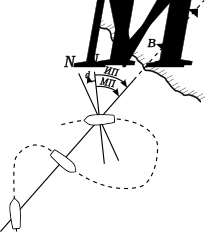
\includegraphics[width=\linewidth]{N014}
  \caption{Определение девиации по створу}
  \label{fig:N14}
\end{figure}

Чтобы обеспечить надёжную работу компасов, производят уничтожение их
девиации при помощи магнитов девиационного механизма в нактоузе
каждого компаса. Работа по \textit{уничтожению
  девиации}\index{девиация!уничтожение} проводится
специалистами\-/девиаторами на оборудованных створами девиационных
полигонах. Уничтожить девиацию полностью невозможно. Поэтому после
проведения работ по уничтожению девиации девиатор приступает к
определению остаточной девиации. Наблюдения проводят на створах,
магнитное направление которых (\MP) известно, на восьми равноотстоящих
курсах \--- главных и четвертных. В момент пересечения створа на
каждом из восьми курсов берут по главному компасу \KP створных знаков
(см. рис.~\ris{N14}). Пользуясь соотношением $\delta = \MP - \KP$
девиатор вычисляет девиацию для восьми курсов, а затем рассчитывать
таблицу остаточной девиации компаса с точностью до 0,1\gr обычно с
интервалом в 10\gr или 15\gr. Полученные данные сводят в
\textit{таблицу девиации}\index{девиация!таблица}. Аргументом для
входа в таблицу (табл.~\ref{tab:N1}) служит \KK судна.

\begin{table}[htb]
  \centering{}
  \begin{tabular}{r|r||r|r}
    \toprule
    $\delta \gr$ & \KK\gr & \KK\gr & $\delta \gr$ \\
    \midrule
    $+1,7$ & 360 &  0 & $+1,7$ \\
    $+1,7$ & 350 & 10 & $+1,7$ \\
    $+1,7$ & 340 & 20 & $+1,7$ \\
    $+1,6$ & 330 & 30 & $+1,8$ \\
    $+1,3$ & 320 & 40 & $+2,0$ \\
    $+1,0$ & 310 & 50 & $+2,1$ \\
    $+0,6$ & 300 & 60 & $+2,3$ \\
    0,0  & 290 & 70 & $+2,5$ \\
    $-0,5$ & 280 & 80 & $+2,6$ \\
    $-1,3$ & 270 & 90 & $+2,7$ \\
    $-2,0$ & 260 & 100 & $+2,6$ \\
    $-2,1$ & 250 & 110 & $+2,4$ \\
    $-2,3$ & 240 & 120 & $+2,0$ \\
    $-2,8$ & 230 & 130 & $+1,5$ \\
    $-2,9$ & 220 & 140 & $+0,8$ \\ 
    $-2,8$ & 210 & 150 & $+1,0$ \\
    $-2,4$ & 200 & 160 & $-0,7$ \\
    $-2,3$ & 190 & 170 & $-1,6$ \\
    $-2,0$ & 180 & 180 & $-2,0$ \\
    \bottomrule
  \end{tabular}
  \caption{Таблица девиации}
  \label{tab:N1}
\end{table}

\section{Поправка магнитного компаса. Исправление и перевод курсов и пеленгов}

Алгебраическая сумма девиации и магнитного склонения, на величину
которой компасные направления отличаются от истинных, называется
\textit{поправкой магнитного компаса}\index{компас!поправка}:

\begin{equation}
  \Delta \MK = \delta + d 
\end{equation}

Девиацию и склонение берут со своими знаками. 

\begin{figure}[!htb]
  \centering{}
  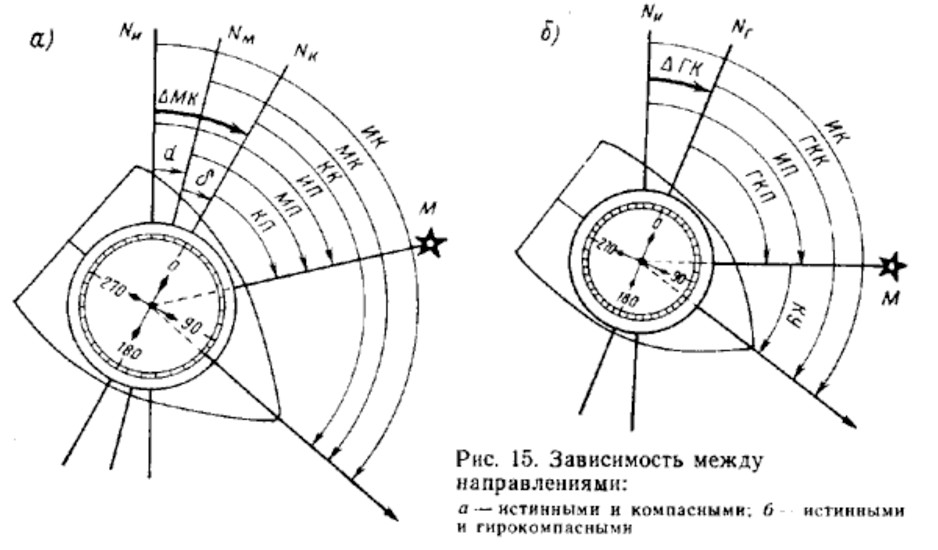
\includegraphics[width=\linewidth]{N015.pdf}
  \caption{Зависимость между истинным и компасным направлениями}
  \label{fig:N15}
  \small
  \centering{}
  % \textit{а} \--- истинным и компасным; \textit{б} \--- истинным и гирокомпасным
\end{figure}

Задачи, связанные с переходом от компасных курсов и пеленгов к
истинным, называются \textit{исправлением румбов}\index{исправление румбов},
а задачи, связанные с переходом от снятых с карты истинных
кусов и пеленгов к компасным \--- \textit{переводом румбов}\index{перевод румбов}. Формулы
исправления румбов:

\begin{gather}
  \IK = \KK + \Delta \MK \\
  \IP = \KP + \Delta \MK \\
  \OIP = \OKP + \Delta \MK 
\end{gather}

Формулы перевода румбов: 

\begin{gather}
  \KK = \IK - \Delta \MK \\
  \KP = \IP - \Delta \MK \\
  \OKP = \OIP - \Delta \MK
\end{gather}

\begin{figure}[htb]
  \centering{}
  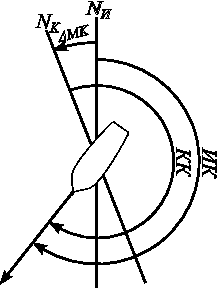
\includegraphics[width=0.5\linewidth]{N016.pdf}
  \caption{Исправление курса}
  \label{fig:N16}
\end{figure}

Для контроля правильности решений навигационных задач бывает полезно
сделать чертёж, чтобы представить себе все соотношения
(рис.~\ris{N16}).

\section{Общие сведения о картографических проекциях}

Если судно, совершая плавание между двумя пунктами, идёт постоянным
курсом, то оно пересекает все меридианы под одним и тем же
углом. Линия, пересекающая все меридианы под постоянным углом,
называется \textbf{локсодромией}\index{локсодромия} (в переводе с
греческого \--- <<кривой бег>>). На поверхности земного шара
локсодромия изображается в виде спирали, стремящейся к полюсу, но
никогда его не достигающей (рис.~\ris{N25}).

\begin{figure}[htb]
  \centering{}
  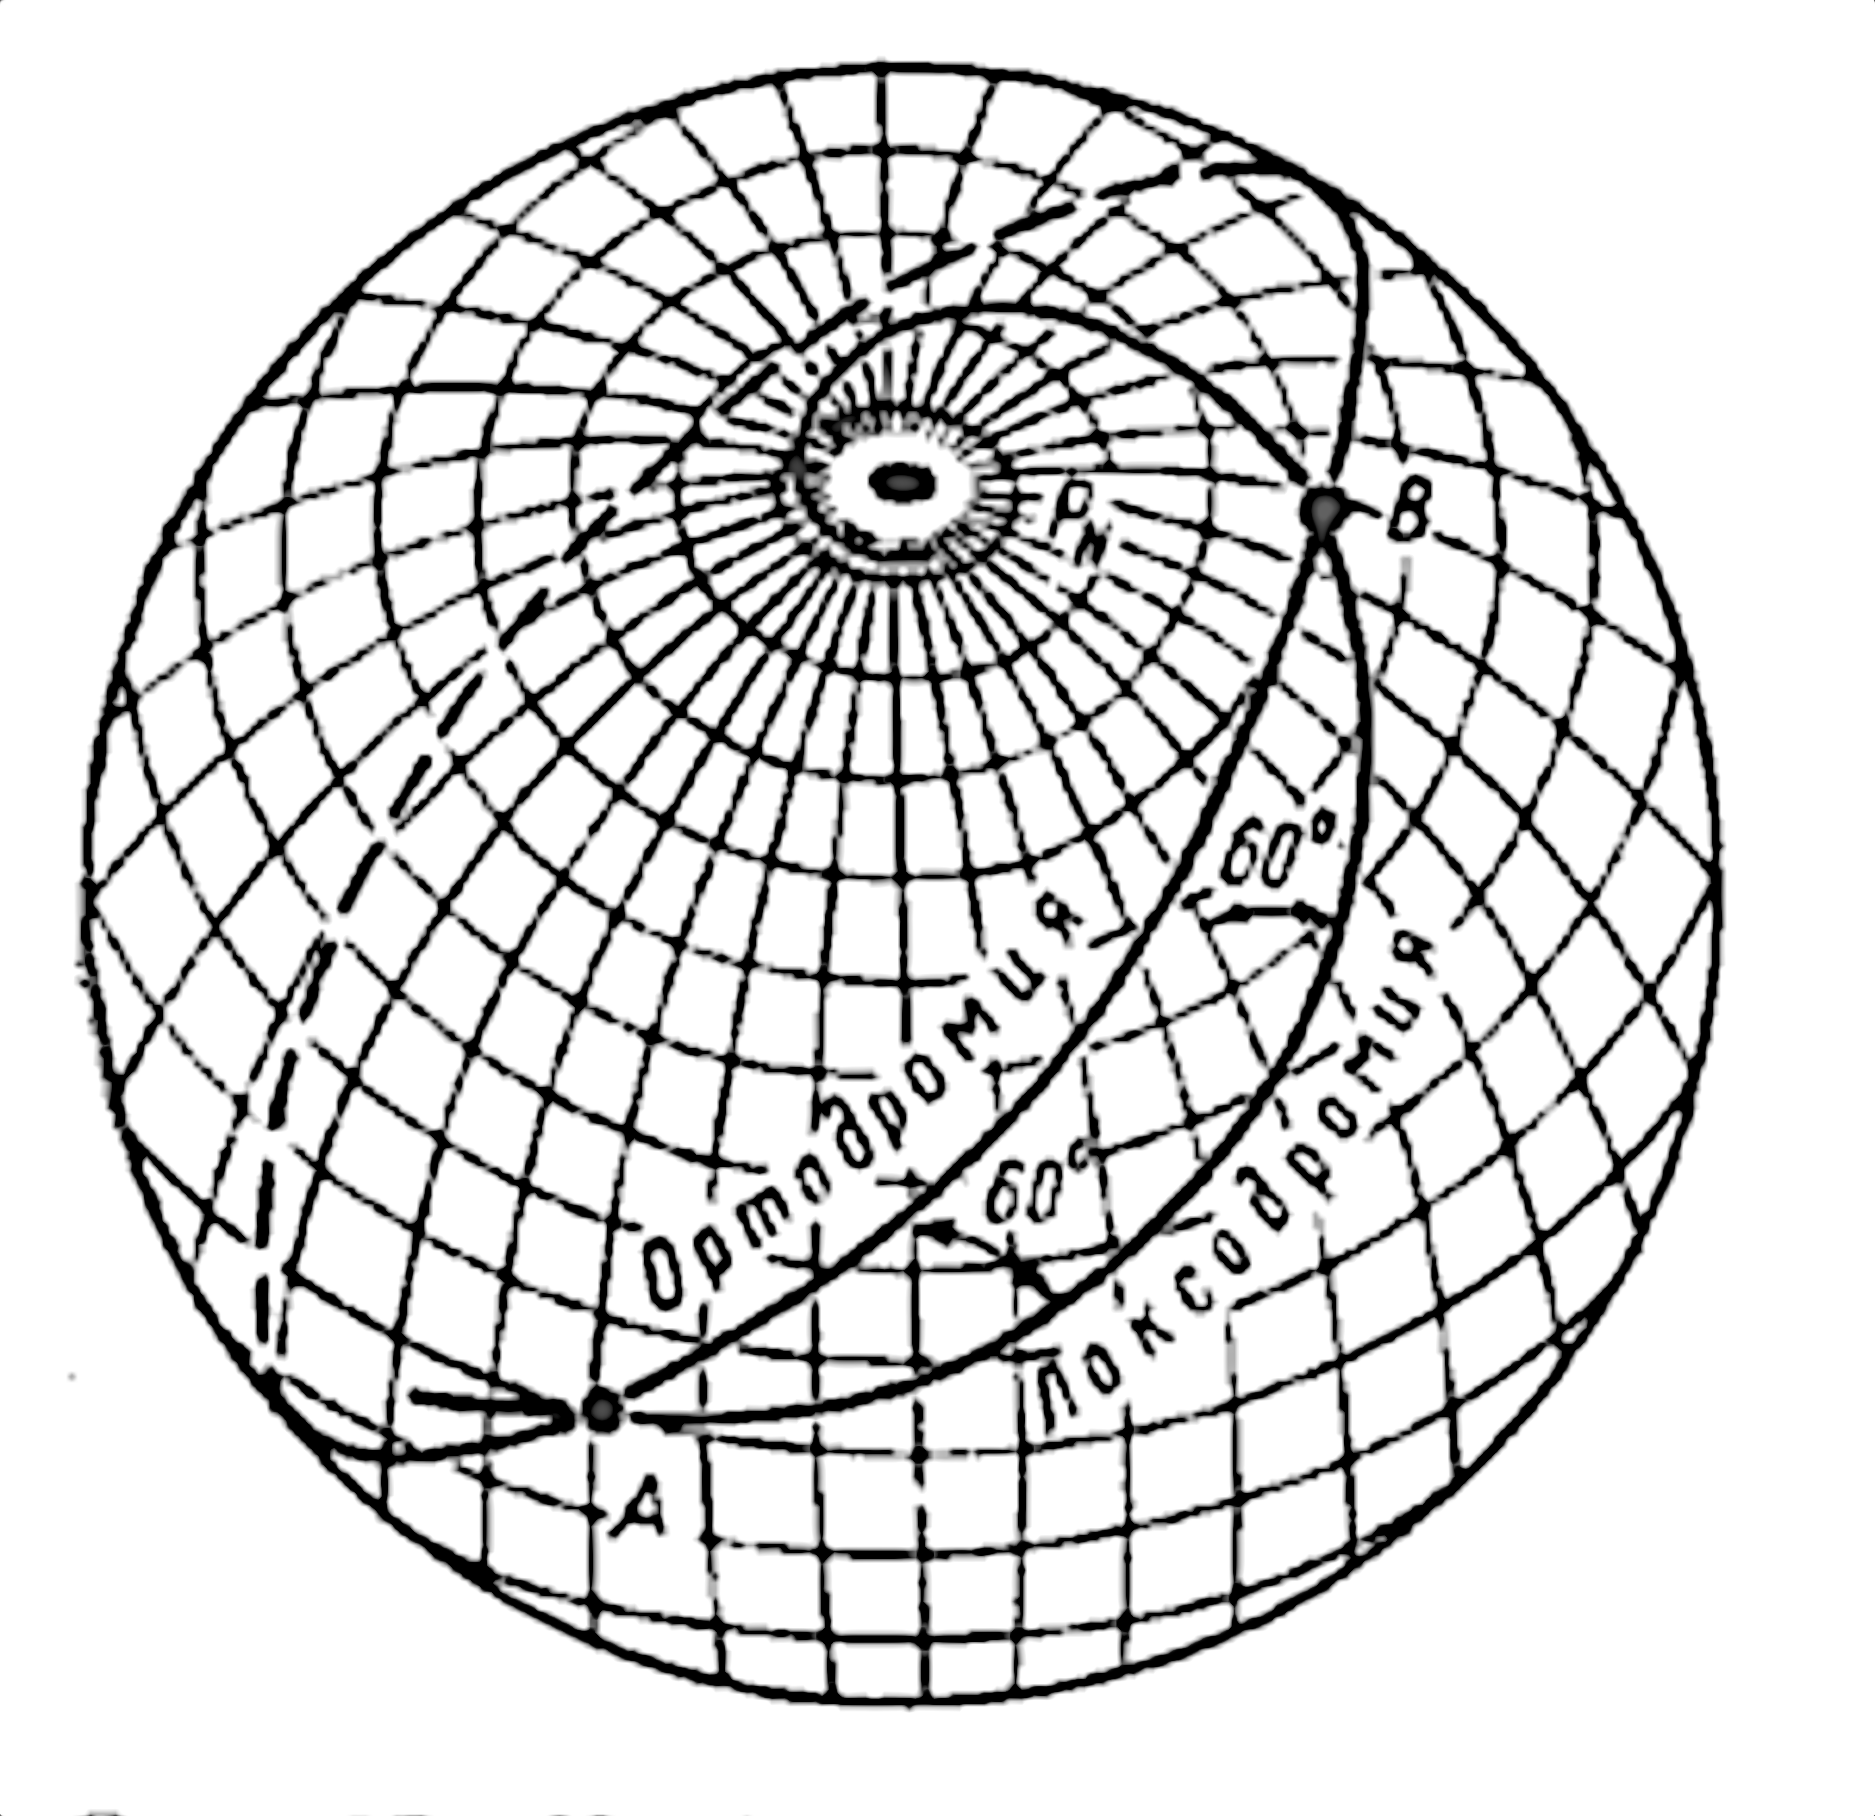
\includegraphics[width=\linewidth]{N025.png}
  \caption{Изображение локсодромии и ортодромии на поверхности Земли}
  \label{fig:N25}
\end{figure}

В частных случаях при плавании курсами 0 и 180\gr локсодромия
совпадает с меридианом, а при плавании курсами 90\gr и 270\gr \--- с
параллелью.

Плавание по локсодромии, т.\=,е. постоянным курсом, удобно. Это
упрощает работу судоводителя. Недостатком плавания по локсодромии
является то, что она не является кратчайшим расстоянием между точками
на земной поверхности. Кратчайшим расстоянием между данными пунктами
на земной поверхности является меньшая дуга большого круга, проходящая
через эти точки или \textbf{ортодромия}\index{ортодромия} (в переводе
с греческого \--- <<прямой бег>>). При небольших переходах разность в
длине между локсодромией и ортодромией незначительна, ею пренебрегают
и совершают плавание по локсодромии.

Морские навигационные карты применяют для графического учёта движения
судна во время его плавания. Для этого на карте прокладывают
локсодромические курсы судна и пеленги на различные ориентиры.

Основные требования, предъявляемые к морской навигационной карте: 

\begin{enumerate}
\item линия курса и пеленгов должны изображаться прямыми
  линиями. Поэтому все меридианы на карте должны быть взаимно
  параллельны, чтобы прямая линия, изображающая линию курса судна,
  пересекала бы их под одним и тем же углом;
\item карта должна быть равноугольной. Это значит, что углы и
  направления, измеренные на местности, должны соответствовать углам и
  направлениям на морской навигационной карте.
\end{enumerate}

Из всех видов картографических проекций в судовождении находят
наибольшее применение \textbf{меркаторская}\index{проекция!меркаторская}
и \textbf{гномоническая}\index{проекция!гномоническая} (центральная).

\begin{figure*}[htb]
  \centering{}
  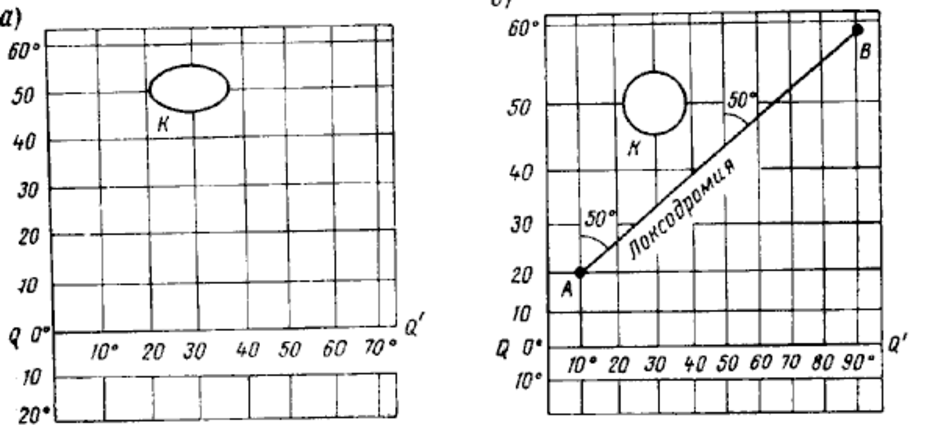
\includegraphics[width=0.8\linewidth]{N028.pdf}
  \caption{Построение меркаторской проекции}
  \label{fig:N28}
  \small
  \centering{}
  \textit{а} \--- сетка меридианов и параллелей; \textit{б} \--- меркаторская проекция
\end{figure*}

\textbf{Масштаб}\index{карты!масштаб} карты определяется как отношение
длины прямой между двумя точками на карте к действительному
горизонтальному расстоянию между этими же точками на
местности. Различают два вида масштаба: числовой (численный) и
линейный.
 
\textbf{Числовой масштаб}\index{карты!масштаб!числовой} \--- дробь,
числитель которой единица, а знаменатель \--- число, показывающее,
скольким единицам длины на местности равна одна единица на карте.

\textbf{Линейный масштаб}\index{карты!масштаб!линейный} может быть
выражен числовым соответствием единиц длины (например, <<3 мили в 1
см>>) или графически. На морских картах линейный масштаб наносят на
вертикальные рамки карты.

При развёртывании сфероидической поверхности Земли на плоскость
возникают искажения, вследствие чего степень уменьшения изображения в
разных частях карты различна. Другими словами, масштаб карты меняется
при переходе от точки к точке.

Масштаб, присущий данной точке карты, называется \textbf{частным}. В
заголовках карт указывается числовой масштаб, близкий к среднему
значению частных масштабов карт данного моря или района. Такой масштаб
называется \textbf{главным}. Минута широты, т.\=,е. линейная величина
1 минуты дуги меридиана, представляет собой морскую милю. Морские мили
будут изображаться на меркаторской карте разными по длине участками
меридианов, увеличивающимися по мере удаления от экватора.

Графическое изображение 1-й морской мили на меркаторской карте на
данной широте называется \textbf{меркаторской
  милей}\index{миля!меркаторская}. Измерять расстояние на карте
следует меркаторскими милями на соответствующей им широте.

\section{Классификация морских карт по назначению. Содержание морских навигационных карт}

\begin{description} 
\item [Планы]\index{карты!планы} (масштаб 1\=,:\-,500 \--- 1\=,:\-,25\=,000)
  предназначены для ориентировки при заходах судов на рейды, в порты,
  бухты и т.\=,д.
\item [Частные карты]\index{карты!частные} (масштаб 1\=,:\-,25\=,000
  \--- 1\=,:\-,50\=,000) предназначены для плавания в районах, сложных
  в навигационном отношении: при проходе узкостей, в шхерах и
  непосредственно у берегов.
\item [Путевые карты]\index{карты!путевые} (масштаб 1\=,:\=,100\=,000
  \--- 1\=,:\=,500\=,000) используют для обеспечения плавания судна в
  значительном удалении от берегов, иногда вне видимости береговых
  ориентиров. Карты этого типа наиболее распространены. Как правило,
  на путевых картах ведётся прокладка пути судна.
\item [Генеральные карты]\index{карты!генеральные} (масштаб
  1\=,:\=,1\=,000\=,000 \--- 1\=,:\=,5\=,000\=,000) используют для
  ведения прокладки при плавании в открытом море в большом удалении от
  берегов, для общего изучения условий перехода и для предварительной
  прокладки.
\end{description}

Побережья морей <<покрываются>> рядом морских карт, каждая из которых
охватывает свой географический район. Для связи с соседними картами и
сохранения непрерывности графического счисления пути судна соседние
карты имеют <<находы>>, т.\=,е. взаимные перекрытия.

Карты печатают на стандартных листах размером $75 \times
100$~см. Кроме того, они могут быть изданы на половине или четверти
стандартного листа размерами соответственно $75 \times 50$ и
$38 \times 50$~см. Если какая-то часть побережья не размещается в
заданном масштабе на стандартном листе, дополнительно к оттиску карты
может быть напечатан клапан на нестандартном листе. Клапан подклеивают
к основному листу карты. Иногда клапан печатают на свободном месте
непосредственно на карте.

Морским картам присваивают пятизначные адмиралтейские номера. Каждая
из цифр номера карты условно обозначает название океана или его части,
тип карты в зависимости от её масштаба, район океана или моря и
порядковый номер карты в данном районе. Особые буквенные или цифровые
обозначения вводят для справочных карт и карт специального назначения.

Картографическая сетка морской карты заполняется в соответствии со
своим назначением географическими и навигационными элементами
содержания, надписями и элементами дополнительной характеристики. К
географическим элементам содержания карты относятся изображения
берегов океанов, морей, заливов, рельефа морского дна и суши,
государственных границ, населённых пунктов. К навигационным элементам
отнесены порты, средства навигационного оборудования, фарватеры,
морские каналы, навигационные опасности, навигационные ориентиры,
данные магнитного склонения и другие элементы карты, имеющие
навигационный характер. Надписи \--- это заголовок карты,
географические названия, различные пояснения и предупреждения, а также
данные об издании и корректуре карты. К элементам дополнительной
характеристики относятся врезки, т.\=,е. небольшие крупномасштабные
планы или карты важных в навигационном отношении участков побережья,
помещённые на свободных местах листа, таблицы со сведениями о приливах
и течениях, рисунки маяков, знаков и т.\=,д.
 
Элементы содержания карт передаются условными знаками, символами
изображения или схематическими рисунками объектов. Различного рода
надписи на картах, относящиеся к цвету и характеру огней, наименованию
грунтов и т.\=,д., дают в виде сокращений. Местоположение объектов, не
выражаемых в масштабе карты, показывается условными
обозначениями. Действительное место объекта при этом принимается в
геометрическом центре знака, если он имеет правильную геометрическую
форму, или в середине основания, если объект изображается
несимметричным рисунком или знаком с широким основанием.

Глубины приводятся к нулю глубин и даются в метрах и дециметрах,
причём глубины от 0 до 5~м округляют с точностью до 0,1~м; от 5 до 20
м \--- до 0,2~м; 20 и более \--- до 1~м. Кроме нанесения отметок
глубин, на картах проводят линии равных глубин \--- изобаты. Изобата
10~м считается предостерегательной для малых судов, а 20~м \--- для
крупнотоннажных.

Береговую линию в морях с приливами наносят на карту двумя
линиями. Одна из них (основная) соответствует следу полной воды в
сизигию, а другая \--- наинизшему уровню моря. Заключённая между этими
линиями зона называется осушкой. В морях, где приливы не превышают
0,5~м, за береговую линию принимают урез воды при среднем уровне моря.

Высоты маяков и знаков в морях, не имеющих приливов, даются над
средним уровнем моря, а в морях со значительным приливом \--- над
уровнем средней полной сизигийной воды.

Средства навигационного оборудования (СНО) \--- маяки, светящие и
несветящие знаки, знаки створов, радиомаяки, плавучие маяки, буи, вехи
\--- показывают на картах внемасштабными условными знаками. Рядом с
изображением светящих СНО с помощью сокращений надписывают их
характер, количество проблесков или затмений, период дальность
видимости огня, сведения о радиотехнических станциях, туманных
сигналах, секторах освещения. Направления и сектора маяков дают
истинные, считая с берега от 0 до 360\gr по часовой стрелке. Рядом с
изображением несветящих знаков в виде дроби показывают их высоту от
уровня моря (числитель) и от основания знака (знаменатель). Рядом с
изображением буев указывают их окраску, звуковые сигналы, порядковые
номера, данные о радиолокационном отражателе, а у светящих буев \---
также и характер огня. Через центры изображений створных знаков
проводят створные линии, ходовую часть которых изображают сплошной
линией, неходовую \--- пунктиром.

Так как степень подробности изображения местности зависит от масштаба
карты, то из всех карт, имеющихся на данный район, всегда следует
пользоваться картой самого крупного масштаба. Чтение карты начинают с
её заголовка, в котором указывают название изображаемого района моря,
масштаб карты, сведения о нуле глубин, принятые единицы для указания
глубин и высот предметов, данные о магнитном склонении. Затем должны
быть прочитаны напечатанные на карте предупреждения и примечания,
установлены даты издания, а также большой и малой корректур. Для
получения возможно полного представления об изображённой на карте
местности изучают все показанные на ней географические и навигационные
элементы изображения.

При плавании в сложных в навигационном отношении районах рекомендуется
сделать подъём карты\index{подъём карты}, т.\=,е. увеличить её
наглядность выделением наиболее важных элементов карты. Для этого, в
частности, карандашом наносят дуги, соответствующие дальности
видимости маяков, заштриховывают опасные сектора огней, проводят линии
опасных пеленгов. Перед пользованием картой нужно оценить её с точки
зрения достоверности и полноты нанесённого на неё изображения. Чем
позднее составлена карта, тем больше ей можно доверять. Об уровне
современности карты судят также по датам её нового издания, большой и
малой корректур. Для оценки достоверности изображения рельефа дна
устанавливают степень подробности промера. Хорошо обследованным
районам моря соответствует на карте большая частота и равномерность
нанесения глубин. Редко и неравномерно показанные глубины, белые пятна
между ними являются признаком недостаточной изученности района.

\section{Графические задачи, решаемые на морских картах}

Все построения в процессе графического счисления выполняют при помощи
прокладочного инструмента: навигационного транспортира, параллельной
линейки, циркуля\-/измерителя, чертёжного циркуля с карандашом. Линии
наносят простым карандашом и убирают мягкой резинкой.

\textbf{Снять с карты координаты заданной точки.} Наиболее точно эту
задачу можно выполнить с помощью циркуля\-/измерителя. Для снятия
широты одну ножку циркуля ставят в заданную точку, а другую так
подводят к ближайшей параллели, чтобы описанная циркулем дуга её
касалась. Не изменяя угла раствора ножек циркуля, подносят его к
вертикальной рамке карты и ставят одну ножку на параллель, до которой
измерялось расстояние. Другую ножку ставят на внутреннюю половину
вертикальной рамки в сторону заданной точки и снимают отсчёт широты с
точностью до 0,1 наименьшего деления рамки. Долготу заданной точки
определяют таким же образом, только расстояние измеряют до ближайшего
меридиана, а отсчёт долготы снимают по верхней или нижней рамке карты.

\textbf{Нанести точку по заданным координатам.} Работу выполняют
обычно с помощью параллельной линейки и циркуля\-/измерителя. Линейку
прикладывают к ближайшей параллели и отодвигают одну её половину до
заданной широты. Затем раствором циркуля берут расстояние от
ближайшего меридиана до заданной долготы по верхней или нижней рамке
карты. Одну ножку циркуля ставят у среза линейки на тот же меридиан, а
другой ножкой делают слабый укол также у среза линейки в сторону
заданной долготы. Место укола и будет являться заданной точкой.

\textbf{Измерить расстояние между двумя точками на карте или отложить
  известное расстояние от заданной точки.} Если расстояние между
точками небольшое и может быть измерено одним раствором циркуля, то
ножки циркуля ставят в одну и другую точки, не меняя его раствора,
приставляют к боковой рамке карты в той же примерно широте, в которой
лежит измеряемое расстояние. Большое расстояние при измерении
разбивают на части. Каждую часть расстояния измеряют милями в широте
данного участка. Можно также раствором циркуля взять с боковой рамки
карты <<круглое>> число миль (10, 20 и т.\=,д.) и сосчитать, сколько
раз уложить это число по всей измеряемой линии. При этом мили снимают
с боковой рамки карты примерно против середины измеряемой
линии. Остаток расстояния измеряют обычным способом. Если нужно
отложить от заданной точки небольшое расстояние, то его снимают
циркулем с боковой рамки карты и откладывают на проложенной
линии. Расстояние берут с рамки примерно в широте заданной точки с
учётом его направления. Если откладываемое расстояние большое, то
берут с рамки карты примерно против середины заданного расстояния 10,
20 миль, и т.\=,д. и откладывают нужное число раз. От последней точки
отмеряют остаток расстояния.
 
\textbf{Измерить направление проложенной на карте линии истинного
  курса или пеленга.} Параллельную линейку прикладывают к линии на
карте и приставляют к срезу линейки транспортир. Транспортир
перемещают вдоль линейки до тех пор, пока его центральный штрих не
совпадёт с каким-либо меридианом. Деление на транспортире, через
которое проходит тот же меридиан, соответствует направлению курса или
пеленга. Так как на транспортире нанесены два отсчёта, то при
измерении направления проложенной линии следует учитывать четверть
горизонта, в которой лежит заданное направление.

\textbf{Проложить от заданной точки линию истинного курса или
  пеленга.} При выполнении этой задачи используют транспортир и
параллельную линейку. Транспортир накладывают на карту так, чтобы его
центральный штрих совпал с каким-либо меридианом. Затем транспортир
поворачивают в ту и другую сторону до тех пор, пока с тем же
меридианом не совпадёт штрих дуги, соответствующей отсчёту заданного
курса или пеленга. К нижнему срезу линейки транспортира прикладывают
параллельную линейку, и, убрав транспортир, раздвигают её, подводя к
заданной точке. По срезу линейки в нужную сторону проводят
линию. Перенести точку с одной карты на другую. С карты снимают
направление и расстояние до заданной точки от какого-либо маяка или
другого ориентира, нанесённого на обе карты. На другой карте, проложив
от этого ориентира нужное направление и отложив по нему расстояние,
получают заданную точку. Эта задача является комбинированной.

\section{Графическое счисление пути судна}

Для того чтобы судить о безопасности плавания, ориентироваться в
окружающей обстановке и правильно выбирать курсы для дальнейшего
перемещения, судоводитель должен в любой момент знать положение своего
судна. Для этого он ведёт \textbf{навигационную прокладку}
\index{прокладка!навигационная}.

Перед выходом судна в рейс под руководством капитана по картам и
навигационным пособиям изучают условия плавания на всем предстоящем
переходе. На основании этих данных выполняют \textbf{предварительную
  прокладку} \index{прокладка!предварительная}. Однако она даёт только
общее представление об условиях перехода. С момента выхода в рейс
окончательный выбор курсов и все принимаемые к учёту факторы
определяются конкретной обстановкой плавания. Поэтому в рейсе
осуществляют \textbf{исполнительную прокладку}
\index{прокладка!предварительная}. Она включает в себя счисление пути,
расчёты и построение на карте, расчёты маневрирования для расхождения
с другими судами.

\textbf{Счислением}\index{счисление}\index{обсервация} называется
непрерывный учёт элементов движения судна (скорости и направления) и
воздействий внешних сил с целью определения координат судна
(счислимого места) без наблюдений береговых ориентиров и небесных
светил (обсерваций). Этот учёт осуществляют на основании значений
курса, скорости и вектора сноса судна. Исходную точку для счисления на
карте определяет капитан. За такую точку могут быть приняты точное
место судна, полученное сразу же после выхода за пределы акватории
порта, плавучий маяк, приёмный буй и т.д. Её координаты записывают в
судовой журнал. К моменту начала исполнительной прокладки следует
включить лаг, определить поправку компаса по створам или другим
способом.

\section{Ведение счисления при плавании без дрейфа и течения}

При плавании без дрейфа и течения линия пути судна на карте совпадает
с линией \IK, поэтому учёт перемещения судна на карте производится по
линиям \IK, по которым откладывают расстояния, пройденные судном по
лагу с учётом его коэффициента \cidx{K}{Л}. От исходной точки на карте
прокладывают линию первого курса. Снятый с карты \IK переводят в \KK,
на который ложатся по магнитному компасу. На карте над линией \IK
надписывают курс по компасу и его поправку. Пройденное по курсу
расстояние \cidx{S}{Л} определяют по лагу:
%
\begin{equation}
  \cidx{S}{Л} = \cidx{K}{Л} \cdot (\mcyr{ОЛ}_2 - \mcyr{ОЛ}_1) \label{eq:SL}
\end{equation}
%
где $\mcyr{ОЛ}_2$ \--- отсчёт лага в точке нахождения судна,
$\mcyr{ОЛ}_1$ \--- отсчёт лага в исходной точке, \cidx{K}{Л} \---
коэффициент лага.
 
На линии \IK в указанных ниже случаях наносят счислимое мести судна,
т.\=,е. место, рассчитанное по курсу и плаванию. Если плавание
совершают вблизи берегов, \textit{счислимые точки}\index{счислимые точки}
отмечают каждый час, в открытом море \--- в конце
вахты. Кроме того, счислимое место наносят в точках начала и конца
поворотов, при изменении скорости, при получении обсерваций. Рядом с
местом судна в виде дроби записывают момент по судовым часам с
точностью до 1 мин ($T$) и отсчёт лага с точностью до 0,1 мили
(\mcyr{ОЛ}). (См.рис~\ris{N31}).

\begin{figure}[htb]
  \centering{}
  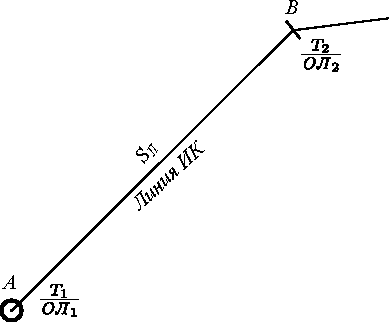
\includegraphics[width=0.8\linewidth]{N031.pdf}
  \caption{Расчёт счислимого места при прокладке}
  \label{fig:N31}
\end{figure}

В реальных условиях морского плавания возможны три основных варианта,
определяющих соответствующие практические приёмы счисления пути яхты:

\begin{enumerate}
\item плавание в условиях устойчивого полного ветра; 
\item плавание в условиях устойчивого противного ветра; 
\item плавание при неустойчивом по силе и направлению ветре. 
\end{enumerate}

В первом случае яхту ведут обычно по линии пути, проложенного при
предварительной прокладке. Условия счисления здесь благоприятные. Во
втором случае выполняют лавировку относительно генерального курса, при
этом прокладываемый фактический путь на каждом галсе не совпадает с
предварительной прокладкой. Если лавировочный галс не слишком крутой,
то рулевой точно выдерживает заданный курс, что упрощает счисление и
повышает его точность. В таких условиях продолжительность галсов
зависит от угла лавировки (угол между генеральным курсом и путём
яхты). При равенстве углов правого и левого галсов их
продолжительность одинакова, а лавировка может быть симметричной. Если
нет \--- счисление и прокладку пути выполняют на каждом частном
лавировочном галсе по данным приборов. Если лага нет, скорость
рекомендуется оценивать на каждом галсе.
 
При лавировке может случиться, что рулевой по указанию капитана яхты,
выбираясь на ветер, не обращает внимания на компас. Здесь через
небольшие, но равные промежутки времени (15\otdo 30~мин.) определяют и
записывают средний \KK и соответствующий ему \IK, по которому
откладывают данные, полученные по лагу или скорости. При неустойчивом
ветре курс рулевому не задают, а ставят задачу править по парусу в
поисках ветра, придерживаясь по возможности ближе к генеральному
курсу. Иногда в такой ситуации в зависимости от местных признаков и
прогноза погоды бывает выгодно уклониться от генерального курса, чтобы
скорее получить полный устойчивый ветер (например, бриз\index{бриз} под
берегом). Во всех этих случаях в интересах счисления пути на яхте
фиксируют все повороты и на каждом галсе (в начале и конце галса
обязательно) с определённой периодичностью (1\otdo 2 раза в час, в
зависимости от условий) записывают данные о движении судна (время,
курс, скорость, отчёт лага). Эти записи обрабатывают, усредняя курс и
скорость каждого галса, а затем прокладывают на карте.

Практика показывает, что точность счисления в таких условиях
повышается с увеличением дискретности наблюдений. Ошибки аппроксимации
криволинейных участков плавания прямолинейными будут незначительны по
сравнению с другими ошибками.

\section{Дрейф судна}

В навигации дрейфом \index{дрейф} ($\alpha$) называют снос судна с
линии курса под совместным действием ветра и вызванного им
волнения. При дрейфе судно перемещается относительно воды под
совместным действием судовых машин и ветра. Линия его фактического
перемещения ($OB$), называемая линией пути судна при дрейфе, не
совпадает с курсом судна ($OA$). (См.рис~\ris{N33}). При смещении
линии пути вправо от \textit{ДП} судна (ветер дует в левый борт) a
приписывают знак плюс ($+$), а при смещении влево (ветер дует в правый
борт) \--- знак минус ($-$).

\begin{figure}[htb]
  \centering{}
  \includegraphics[width=\linewidth]{N033.pdf}
  \caption{Дрейф судна}
  \label{fig:N33}
\end{figure}

Зависимость между путевым углом с учётом дрейфа ($\mcyr{ПУ}_\alpha$),
\IK и $\alpha$:

\begin{gather} 
  \mcyr{ПУ}_\alpha = \IK + \alpha ; \\
  \IK = \mcyr{ПУ}_\alpha - \alpha ; \\
  \alpha = \mcyr{ПУ}_\alpha - \IK 
\end{gather}

Угол дрейфа может быть определён путём сравнения действительного пути
судна, полученного по обсервациям, с \IK.

При следовании в виду берегов проводят ряд надёжных навигационных
наблюдений. Соединив обсервованные точки, получают линию
действительного перемещения судна, т.\=,е. линию пути при дрейфе
$\mcyr{ПУ}_\alpha$ (рис.~\ris{N34}). Угол между линией пути и
проложенной на карте линией \IK соответствует углу дрейфа. Найденный
угол дрейфа с его знаком учитывают при дальнейшем счислении. Если в
районе плавания имеется течение, то полученный угол сноса будет
результатом воздействия на судно не только ветра, но и течения.

\begin{figure}[htb]
  \centering{}
  \includegraphics[width=0.8\linewidth]{N034.pdf}
  \caption{Определение угла дрейфа}
  \label{fig:N34}
\end{figure}

\section{Учёт дрейфа при счислении}

Если судно испытывает дрейф, то при ведении прокладки на карту наносят
линию пути судна при дрейфе.

На ней надписывают \KK, поправку компаса и принятый к учёту угол
дрейфа $\alpha$ со своим знаком. По линии пути откладывают пройденные
по лагу расстояния \cidx{S}{Л}. Считается, что при $\alpha$ < 8\otdo
10\gr все системы лагов учитывают измерение скорости, вызываемое
ветром. Поэтому плавание судна по лагу рассчитывают, как обычно
(форм.~\ref{eq:SL})

Если судоводитель не уверен в точности угла дрейфа, то для контроля
безопасности плавания, кроме линии пути при дрейфе, на карту
рекомендуется наносить линию \IK. Обе эти линии должны проходить чисто
относительно подводных препятствий. Счисление ведётся только по линии
пути, по которой и происходит перемещение судна.

\section{Морские течения}

\textit{Морскими течениями}\index{морские течения} \index{течение!морское} называют
горизонтальные перемещения больших масс воды. Течение характеризуется
его элементами: направлением и скоростью.

\textbf{Направление течения} \index{направление течения}
\index{течение!направление} \cidx{K}{Т} указывают в градусах по
круговому счету или румбах и задают по той точке горизонта, к которой
течение направлено.

\textbf{Скорость течения} \index{скорость течения}
\index{течение!скорость} $V_T$ измеряют в узлах, а небольшие его
скорости \--- в милях в сутки.

По характеру течения классифицируют на \textbf{постоянные}
\index{течение!постоянное}, элементы которых из года в год почти не
изменяются, \textbf{периодические} \index{течение!периодическое},
элементы которых меняются по определённому закону, и \textbf{временные
  (случайные)} \index{течение!временное} \index{течение!случайное},
элементы которых могут резко меняться.

На практике судоводителю чаще всего приходится иметь дело с
постоянными и периодическими (\textbf{приливно\-/отливными})
\index{течение!приливно-отливное} течениями. Сведения об элементах
постоянных и приливно\-/отливных течений помещают в лоциях, атласах
течений и на картах. При этом указывают средние значения элементов
течений, которые могут значительно отличаться от
действительных. Перемещение судна относительно грунта при плавании на
течении определяют следующими факторами (рис.~\ris{N36}).

\begin{figure}[htb]
  \centering{}
  \includegraphics[width=\linewidth]{N036.pdf}
  \caption{Плавание на течении}
  \label{fig:N36}
\end{figure}

Под действием судовых машин судно перемещается относительно воды по
направлению его \textit{ДП}, т.\=,е. линии истинного курса
$OA$. Скорость судна относительно воды является скоростью \cidx{V}{Л}
показываемой лагом. Одновременно вместе со всей массой воды судно
сносится относительно грунта по направлению течения \textit{ОД} со
скоростью течения $V_T$. В результате относительно грунта судно
перемещается по равнодействующей $OB$ со скоростью, называемой
истинной скоростью судна $V$. При этом \textit{ДП} судна остаётся
параллельной линии \IK. Линия $OB$, по которой перемещается судно под
совместным действием судовых машин и течения, называется линией пути
судна на течении. Положение линии пути относительно истинного
меридиана определяется углом $NOB$, который называется путевым углом
на течении \PUb. Угол $\beta$, заключённый между линией истинного
курса судна $OA$ и линией пути $OB$, называется углом сноса
течением. При сносе судна вправо от его \textit{ДП} (течение
направлено в левый борт) приписывают знак ($+$), а при сносе влево
\--- знак ($-$). Зависимость между \PUb, \IK и $\beta$:

\begin{gather} 
  \PUb = \IK + \beta \\ \IK = \PUb - \beta \\ \beta = \PUb - \IK 
\end{gather}

\section{Счисление при плавании на течении}

\begin{figure}[htb]
  \centering{}
  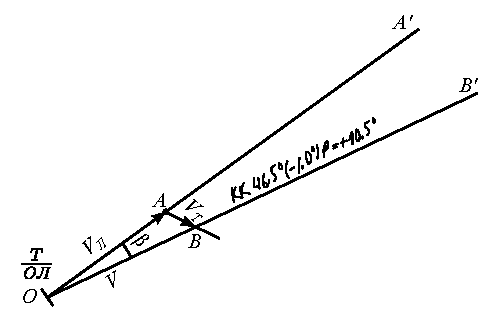
\includegraphics[width=\linewidth]{N037.pdf}
  \caption{Нахождение пути судна при плавании на течении}
  \label{fig:N37}
\end{figure}

При плавании на постоянном течении на карту наносят линию пути судна,
по которой оно фактически перемещается относительно грунта. Над линией
пути надписывают \KK, поправку компаса и угол сноса $\beta$ со своим
знаком. Для вспомогательных расчётов тонкой линией наносят также линию
\IK, по которой откладывают расстояния \cidx{S}{Л}, проходимые судном
относительно воды по показаниям лага. Точки, полученные на линии \IK,
переносят по направлению течения на линию пути (рис.~\ris{N37}). У
счислимых точек на линии пути делают отметку времени и отсчёта лага, а
у соответствующих точек на линии курса \--- только отсчёта лага. Точки
траверза, открытия и скрытия ориентиров наносят на линию пути
(рис.~\ris{N38}).

\begin{figure}[htb]
  \centering{}
  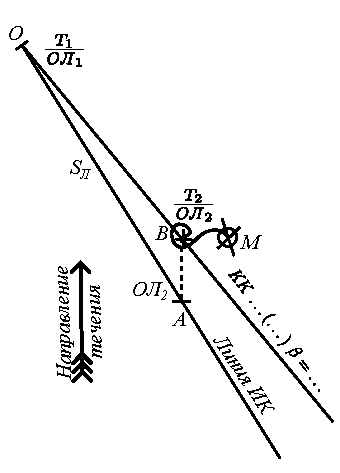
\includegraphics[width=\linewidth]{N038}
  \caption{Счислимое место при плавании на течении}
  \label{fig:N38}
\end{figure}

\section{Счисление при совместном учёте дрейфа и течения}

Рассмотрим случай, когда судно перемещается относительно грунта под
совместным действием судовых машин, ветра и течения. Для ведения
счисления на карте прокладывают линию пути судна при дрейфе и течении
и надписывают \KK, поправку компаса и суммарный угол сноса

\begin{equation}
  c = a + \beta
\end{equation}

Кроме того, для вспомогательных расчётов на карте прокладывают также
линию пути при дрейфе, по которой откладывают плавание судна по лагу
\cidx{S}{Л}. Каждой точке на линии пути при дрейфе соответствует точка
на линии действительного перемещения судна. Эти точки связаны между
собой вектором течения. Графически задачи, связанные с нахождением на
карте линии пути при дрейфе и течении, истинной скорости $V$ и
суммарного угла сноса $c$ по заданным \KK, \cidx{V}{Л}, $a$, и
элементам течения, нанесением счислимого места, предвычислением
времени и \textit{ОЛ} на момент прихода в заданную точку, нахождением траверза
ориентира, решают так же, как и при плавании на течении, но все
вспомогательные построения делают на линии пути при дрейфе, заменяющей
линию \IK.

\section{Оценки точности счисления}

В результате воздействия неучтённых погрешностей действительный путь
судна и пройденное им расстояние (плавание) не будут соответствовать
тем, которые учитывались при счислении на карте, а фактическое место
судна \--- счислимому. Для ориентировочного суждения о погрешностях в
счислении можно пользоваться следующими данными, которые отражают
накопленный обобщённый опыт судовождения и проведённые
исследования. Продолжительности плавания (часы) соответствует
радиальная средняя квадратическая ошибка счисления, \% от $S$: До
3\thr \--- 10\,\%; 3\otdo 6\thr \--- 9\,\%; 6\otdo 10\thr \--- 8\,\%;
10\otdo 14\thr \--- 7\,\%; 14\otdo 18\thr \--- 6\,\%; 18\otdo 23\thr
\--- 5\,\%; 23\otdo 25\thr \--- 4\,\%; более 35\thr \--- 3\,\%.

При прокладке пути судна на карте в том или ином расстоянии от
навигационных опасностей необходимо учитывать возможность отклонения
судна от линии пути, причём значение отклонения будет возрастать с
увеличением пройденного расстояния, в особенности при плавании с
дрейфом и течением. Недостаточная точность счисления вызывает
необходимость дополнительного контроля за местонахождением судна,
т.\=,е. определения его места не только путём счисления, но и по
обсервациям: навигационным, астрономическим либо при помощи GPS.

\section{Определение места судна в море визуальными методами}

Учёт перемещения судна путём ведения графического счисления не
является достаточно точным методом. Для уточнения своего положения
судоводитель должен систематически определять место судна по
наблюдениям различных ориентиров, положение которых известно.

Место, полученное путём обработки результатов таких наблюдений,
называется \textbf{обсервованным}\index{обсервованное место}. Если
обсервованная точка признается надёжной, дальнейшая прокладка ведётся
от этой точки. Несовпадение обсервованной и счислимой точек называют
\textbf{невязкой} \index{невязка}. Значение и направление невязки
рассчитывают при каждой обсервации, так как анализ вызвавших её причин
даёт возможность установить, какие именно ошибки могли быть допущены в
принятых к учёту элементах счисления.

Все величины, которые измеряют с целью определить обсервованное место
судна (пеленги, расстояния, горизонтальные и вертикальные углы),
называют \textbf{навигационными параметрами}
\index{навигационные параметры}. По измеренным
навигационным параметрам рассчитывают и прокладывают на карте изолинии
или заменяющие их линии положения.
\textbf{Навигационной изолинией} \index{навигационная изолиния}
называют линию равных значений навигационного параметра
(рис.~\ris{N40}). Точка пересечения двух таких изолиний и будет местом
судна. На практике всю изолинию не строят, тем более, что на
меркаторских картах она часто имеет вид сложной кривой, а заменяют её
\textbf{линией положения} \index{линия положения}
\--- отрезком прямой, касательной к изолинии вблизи счислимого места.

\begin{figure*}[htb]
  \centering{}
  \includegraphics[width=0.8\linewidth]{N040}
  \caption{Изолинии}
  \label{fig:N40}
  \small
  \centering{}
  \textit{а} \--- при визуальном пеленговании; \textit{б} \--- при измерении горизонтального угла
\end{figure*}

При визуальных способах определения места судна для наблюдений
используют нанесённые на карту хорошо видимые и опознанные береговые и
плавучие маяки, огни, неосвещаемые знаки, башни, церкви, а также
различные естественные ориентиры: мысы, вершины гор, скалы и
т.\=,д. Не следует использовать для обсерваций буи, вехи и другие
знаки плавучего ограждения, так как они могут быть снесены со своих
штатных мест. Для указания на карте места судна, полученного по
обсервациям, применяют условные обозначения
(см. табл.~\ref{tab:signs}).

\begin{table*}[htb]
  \centering{}
  \begin{tabular}[c]{l|c||l|c}
    \toprule
    Общие обозначения & 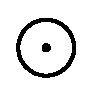
\includegraphics[scale=0.6]{obshie_oboznacheniya.eps} & 
    Счислимо-обсервованное & 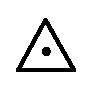
\includegraphics[scale=0.6]{schislimo.eps} \\
    \midrule
    По небесным светилам & 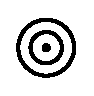
\includegraphics[scale=0.6]{po_nebesnym_svetilam.eps} & 
    Опознанное по глубинам & 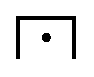
\includegraphics[scale=0.6]{po_glubinam.eps} \\
    \midrule
    С помощью РЛС & 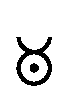
\includegraphics[scale=0.6]{RLS.eps} & 
    Взятое под сомнение & 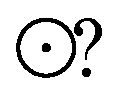
\includegraphics[scale=0.6]{vzyatoe_pod_somnenie.eps} \\
    \midrule
    С помощью радиомаяков & 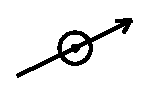
\includegraphics[scale=0.6]{radiomayak.eps} & 
    С помощью РНС & 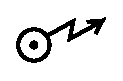
\includegraphics[scale=0.6]{RNS.eps} \\
    \midrule
    Вероятное (осреднённое) & 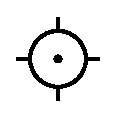
\includegraphics[scale=0.6]{veroyatnoe.eps} & 
    Комбинированное & 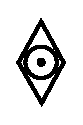
\includegraphics[scale=0.6]{kombinirovannoe.eps}\\
    \midrule
    С помощью навигационных & \\
    спутниковых систем (НСС) & 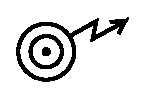
\includegraphics[scale=0.6]{NSS.eps} \\
    \bottomrule
  \end{tabular}
  \caption{Условные обозначения мест, полученных при обсервации}
  \label{tab:signs}
\end{table*}

\section{Определение места судна по пеленгам двух ориентиров}

\begin{figure}[htb]
  \centering{}
  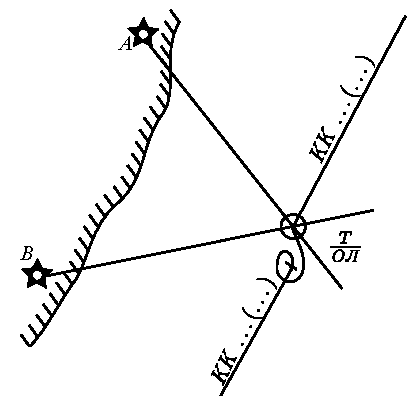
\includegraphics[width=\linewidth]{N041.pdf}
  \caption{Определение места по двум пеленгам}
  \label{fig:N41}
\end{figure}

На берегу выбирают два хорошо видимых и опознанных ориентира $A$ и $B$
(рис.~\ris{N41}) с таким расчётом, чтобы угол между направлениями на
них был по возможности близким к 90\gr, но, во всяком случае, не
меньше 30\gr и не больше 150\gr.

Берут по компасу пеленги ориентиров. Время и \textit{ОЛ} замечают в
момент \textit{Т} вторых наблюдений. Компасные пеленги исправляют
поправкой компаса в истинные и прокладывают на карте. При
незначительных случайных ошибках наблюдений и уверенности в
правильности учитываемой поправки компаса точность определения места
судна по двум пеленгам вполне удовлетворительная. Если угол между
направлениями на ориентиры меньше 30\gr или больше 150\gr, то к
полученному обсервованному месту следует относиться с осторожностью.

\section{Определение места судна по пеленгам трёх ориентиров}

\begin{figure}[htb]
  \centering{}
  \includegraphics[width=\linewidth]{N042.pdf}
  \caption{Треугольник погрешностей}
  \label{fig:N42}
\end{figure}

Три линии положения, проложенные на карте, пересекаются в одной точке
в том случае, если наблюдения, вычисления и прокладка не содержали
никаких ошибок. На практике линии пеленгов часто образуют треугольник,
называемый \textit{треугольником погрешностей} \index{треугольник погрешностей}
($abc$ на рис.~\ris{N42}). Причинами его появления могут быть:

\begin{enumerate}
\item промахи при опознании ориентиров или при взятии отсчётов по
  картушке компаса;
\item случайные ошибки пеленгования. При нормальных условиях
  наблюдений они невелики и не приводят к появлению большого
  треугольника погрешности;
\item ошибки от неодновременного взятия пеленгов. Эти ошибки проявляют
  себя при скорости судна, большей 15\otdo 18~уз, и небольших (2\otdo
  3~мили) расстояниях до ориентиров.
\end{enumerate}

Для установления причин появления треугольника погрешностей проводят
анализ обсервации. Промахи в наблюдениях сразу же обнаруживаются из-за
появления значительного треугольника погрешностей. Чтобы убедиться,
что причиной этого не является промах, измерения пеленгов
повторяют. Если после повторных наблюдений треугольник не уменьшился,
причиной его появления следует считать значительную ошибку в поправке
компаса. Следует изменить её на 2\otdo 4\gr в ту или другую
сторону. Проложив пеленги, исправленные новой поправкой, получают на
карте второй треугольник погрешности ($a'b'c'$ на
рис.~\ris{N42}). Если изменённое значение поправки компаса оказалось
ближе к её истинному значению, то второй треугольник уменьшится по
сравнению с первым и наоборот. Соединив сходные вершины этих
треугольников отрезками прямых, получают в их пересечении точку $M$
(см. рис.~\ris{N42}), которая является обсервованным местом судна,
свободным от влияния систематической ошибки в $\Delta
\MK$. Пользоваться описанным приёмом для нахождения верного места
судна следует только в том случае, если значение сторон треугольника
погрешности 0,5 мили и более. Если его стороны меньше указанного
значения, то вероятное место судна принимают в центре треугольника,
относя причину его возникновения к случайным ошибкам.

\textbf{Практическое выполнение.} Заблаговременно выбирают на берегу
три ориентира с расчётом, чтобы углы между их пеленгами были от 60 до
120\gr. В быстрой последовательности измеряют пеленги каждого
ориентира. При взятии третьего пеленга замечают время и \textit{ОЛ}. Исправляют
пеленги поправкой компаса и прокладывают на карте, принимая место
судна в точке их пересечения. При получении треугольника погрешности
находят верное место судна, как указывалось выше. Снимают с карты
координаты обсервованного места, а также направление и невязку. Эти
данные записывают в судовой журнал. Способ определения места судна по
трём пеленгам является одним из наиболее точных в судовождении.

\section{Определение места судна по двум горизонтальным углам}

\begin{figure*}[!h]
  \centering{}
  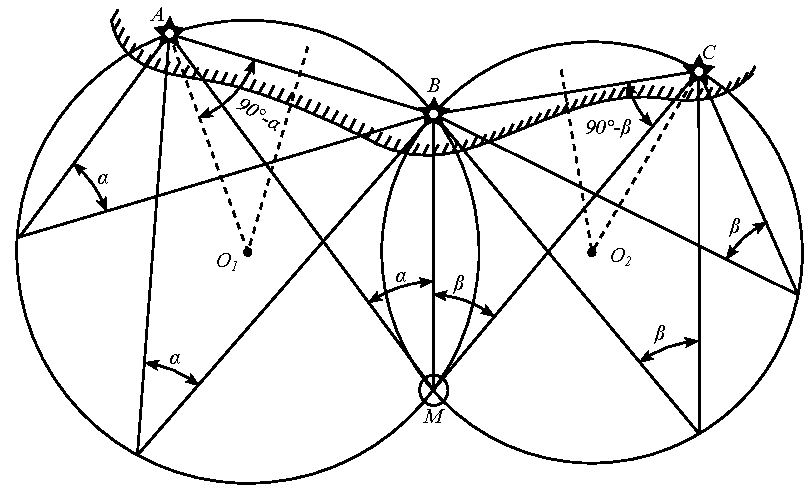
\includegraphics[width=0.8\linewidth]{N043.pdf}
  \caption{Определение места по двум горизонтальным углам}
  \label{fig:N43}
\end{figure*}

Если на берегу имеются три ориентира $A$, $B$ и $C$
(см. рис.~\ris{N43}), то с судна могут быть одновременно измерены два
горизонтальных угла: $\alpha$ \--- между ориентирами $A$ и $B$ и
$\beta$ \--- между $B$ и $C$.

В результате будут получены две окружности \--- изолинии, в одной из
точек пересечения которых (точка $M$) находится судно.

\begin{figure}[!h]
  \centering{}
  \includegraphics[width=\linewidth]{N044.pdf}
  \caption{Использование кальки}
  \label{fig:N44}
\end{figure}

На практике окружности на карту не наносят, а для нахождения места
судна используют кальку (рис.~\ris{N44}). Место судна получают, делая
в точке $M$ нажим карандашом или укол циркулем.

\begin{figure}
  \centering{}
  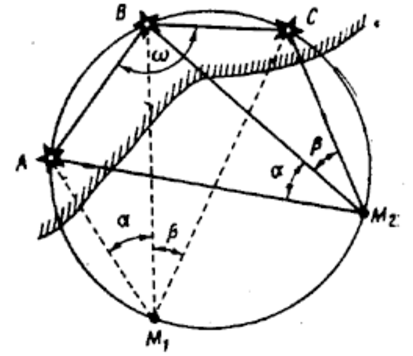
\includegraphics[width=\linewidth]{N045.pdf}
  \caption{Случай неопределённости}
  \label{fig:N45}
\end{figure}

\textbf{Случай неопределённости.} Определение места судна по двум
горизонтальным углам оказывается невозможным, если в момент измерения
углов судно будет находиться на окружности, проходящей через все три
ориентира $A$, $B$, $C$ (рис.~\ris{N45}). Случая неопределённости не
будет, если средний ориентир расположен ближе к судну, чем крайний;
все три ориентира расположены на одной прямой; все три ориентира
находятся на одинаковом расстоянии от судна.

\textbf{Практическое выполнение.} Углы между ориентирами, как правило,
измеряют секстаном. Углы между ориентирами можно определить и при
помощи компаса. Для этого в быстрой последовательности берут пеленги
трёх ориентиров, а затем вычисляют разности между отсчётами смежных
компасных пеленгов: левого и среднего, среднего и правого
ориентиров. Этим приёмом пользуются, в частности, если поправка
компаса ненадёжна.

Определение места судна по двум горизонтальным углам относится к числу
наиболее точных визуальных способов.

\section{Определение места судна по пеленгу и горизонтальному углу}

Этот приём является разновидностью способа определения места судна по
двум пеленгам. Его применяют, когда один из двух ориентиров
почему-либо не виден наблюдателю, расположенному у компаса, например,
закрыт надстройкой. В этом случае измерения обычно проводят два
наблюдателя. Первый располагается так, чтобы видеть оба ориентира,
второй находится у компаса. Первый наблюдатель секстаном измеряет
горизонтальный угол между ориентирами, а второй по команде, подаваемой
в момент измерения угла, берет пеленг. Одновременно замечают время и
\textit{ОЛ}. Отсчёт компасного пеленга исправляют $\Delta \MK$. Для
получения истинного пеленга на второй ориентир к первому пеленгу
прибавляют измеренный угол. Угол берётся со знаком плюс ($+$), если он
был измерен вправо от линии измеренного пеленга, и со знаком минус
($-$), если влево. Место судна получают в пересечении линий двух
истинных пеленгов. Точность обсервации может быть принята равной
точности определения места по двум пеленгам.

\section{Определение места судна по крюйс-пеленгу}


\begin{figure}[htb]
  \centering{}
  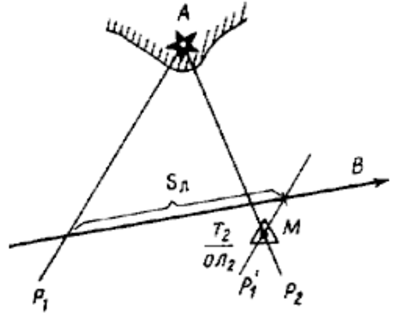
\includegraphics[width=\linewidth]{N046.pdf}
  \caption{Определение места по крюйс-пеленгу}
  \label{fig:N46}
\end{figure}

Если с движущегося судна виден только один ориентир, расстояние до
которого не может быть измерено, то для определения места применяют
способ крюйс\-/пеленга. При этом ориентир пеленгуют 2 раза в различные
моменты времени, место судна получают на момент вторых наблюдений. На
карте счислимо\-/обсервованное место обозначают треугольником.

Наблюдения, вычисления и прокладку при определении места судна по
крюйс\-/пеленгу выполняют в следующем порядке.

Берут первый компасный пеленг ориентира, замечая время и
\textit{ОЛ}. Когда направление на ориентир изменится на 30\otdo 40\gr,
берут второй пеленг и вновь замечают время и \textit{ОЛ}. Компасные
пеленги исправляют поправкой компаса и рассчитывают пройденное судном
расстояние между измеренными пеленгами. Линии истинных пеленгов
прокладывают на карте (см. рис.~\ris{N46}). От точки пересечения
первого пеленга с линией \IK. откладывают по курсу отрезок
\cidx{S}{Л}, через конец которого проводят линию, параллельную первому
пеленгу. В точке пересечения этой линии со вторым пеленгом получают
счислимо\-/обсервованное место судна на момент вторых наблюдений. Если
счисление переносят в полученную точку, то снимают её координаты,
величину и направление невязки, которые записывают в судовой
журнал. Если при счислении учитывали дрейф, то \cidx{S}{Л} откладывают
не по линии \IK, а по линии пути судна при дрейфе
(см. рис.~\ris{N47}), а при течении откладывают \cidx{S}{Л} по линии
пути при течении.

\begin{figure}[htb]
  \centering{}
  \includegraphics[width=\linewidth]{N047.pdf}
  \caption{Крюйс-пеленг на течении}
  \label{fig:N47}
\end{figure}

Точность счислимо\-/обсервованного места зависит от случайных ошибок
пеленгования, соответствия принятой поправки компаса её
действительному значению и от ошибок счисления за время между
моментами взятия пеленгов. Причиной появления ошибок счисления
являются погрешности в показаниях компаса и лага, а также неточный
учёт дрейфа и течения.

Для повышения точности стараются взять второй пеленг как можно быстрее
после первого, однако не ранее того момента, когда он не изменится на
30\otdo 40\gr. При этом пеленгование ведут с таким расчётом, чтобы
второй пеленг ориентира был взят вблизи его траверза.

\section{Определение места судна по пеленгу и расстоянию}

\begin{figure}[htb]
  \centering{}
  \includegraphics[width=\linewidth]{N048.pdf}
  \caption{Определение расстояния до ориентира}
  \label{fig:N48}
\end{figure}

\textbf{Определение расстояния до ориентира.} Расстояние до ориентира
в настоящее время, как правило, определяют с помощью РЛС. В качестве
резервного может быть рассмотрен способ определения расстояния по
вертикальному углу, измеренному секстаном. Определить расстояние по
вертикальному углу можно, если известна высота ориентира над уровнем
моря или его высота над основанием. Предположим, что, находясь в точке
$M$, наблюдатель видит ориентир, высота которого $h$ над уровнем моря
известна (см. рис.~\ris{N48}). Измерив вертикальный угол $\alpha$,
можно рассчитать расстояние $D$ до ориентира. При этом высотой глаза
наблюдателя $e$ можно пренебречь. Тогда из прямоугольного треугольника
$M'OA$ получаем:

\begin{equation}
  D = h \ctg \alpha 
\end{equation}

Выражая $h$ в метрах и $D$ в милях, получим: 

\begin{equation}
  D = \frac{h}{1852} \ctg \alpha 
\end{equation}

Перед измерением вертикального угла подготавливают секстан к
наблюдениям, определяют поправку индекса. Из навигационного пособия
выбирают высоту ориентира над уровнем моря или от
основания. Измеренный угол исправляют поправкой индекса и
инструментальной поправкой ($t + s$). Точность измерения расстояния
рассматриваемым способом невелика. Возможные ошибки связаны с
колебаниями уровня моря и значительное удаление ориентира от береговой
черты.

\begin{figure}[htb]
  \centering{}
  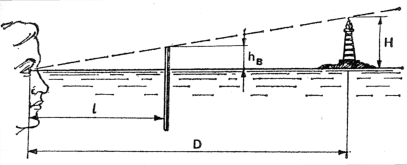
\includegraphics[width=\linewidth]{0082P}
  \caption{Определение расстояния по высоте предмета с помощью линейки}
  \label{fig:N48-1}
\end{figure}

Существует также проверенный практикой способ определения расстояния с
помощью школьной линейки (см. рис.~\ris{N48-1}).

Если известны высота ориентира $H$ (м), длина вытянутой руки $l$ (см)
и видимая высота ориентира \cidx{h}{В} (см), наблюдаемая на шкале
линейки на вытянутой руке, то расстояние от судна до ориентира $D$
(мили) будет равно:

\begin{equation}
  D = \frac{ H \cdot l}{1852 \cdot \cidx{h}{В}} 
\end{equation}

\textbf{Определение места судна по пеленгу и расстоянию.} Этот способ
применяют, если с судна виден только один ориентир $A$, расстояние до
которого может быть определено по измеренному вертикальному углу либо
при помощи РЛС. Изолиниями, в пересечении которых принимается
обсервованное место, являются проложенная на карте линия истинного
пеленга ориентира $AP$ и дуга окружности (засечка), проведённая
радиусом, равным измеренному расстоянию $d$ (рис.~\ris{N49}).

Для уменьшения ошибки от перемещения судна первым измеряют
вертикальный угол, а затем пеленг на момент времени $T$. Для повышения
точности обсервации следует выбирать ориентир, расположенный ближе к
судну. При уверенности в принятой поправке компаса обсервованное место
судна можно считать достаточно надёжным.

\begin{figure}[htb]
  \centering{}
  \includegraphics[width=\linewidth]{N049.pdf}
  \caption{Определение места по пеленгу и расстоянию}
  \label{fig:N49}
\end{figure}

\textbf{Определение места судна по двум расстояниям.} Аналогично
определяется место по двум расстояниям (см. рис.~\ris{N50}). При
помощи РЛС, либо измеряя секстаном вертикальные углы, измеряют
расстояние до двух ориентиров, причём момент времени засекается при
измерении расстояния к ориентиру, который расположен под меньшим углом
к \textit{ДП} судна, и откладывают засечки дуг окружностей на карте,
находя их пересечение, соответствующее месту судна.

\begin{figure}[htb]
  \centering{}
  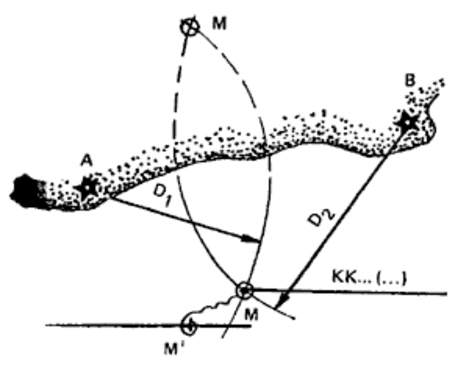
\includegraphics[width=\linewidth]{N050.pdf}
  \caption{Определение места по двум расстояниям}
  \label{fig:N50}
\end{figure} 

\section{Опознание места судна по пеленгу в момент открытия ориентира, по пеленгу и глубине}

Опознанное место в отличие от обсервованного является
ориентировочным. Судоводитель не должен полагаться на него в своих
расчётах, однако его необходимо принимать во внимание, особенно если
оно находится ближе к опасности, чем счислимая точка.

Опознание места по пеленгу в момент открытия ориентира применяют при
подходе к берегу, когда на судне продолжительное время не имели
обсерваций. Заблаговременно рассчитывают дальность видимости ориентира
и ведут наблюдение в направлении, по которому он должен открыться. В
момент обнаружения ориентира берут его компасный пеленг, замечают
время и \textit{ОЛ}. Исправленный пеленг прокладывают на карте. Место
судна получают на линии пеленга, отложив по нему рассчитанное
расстояние. Точность опознанного места во многом зависит от состояния
атмосферы.

\begin{figure}[htb]
  \centering{}
  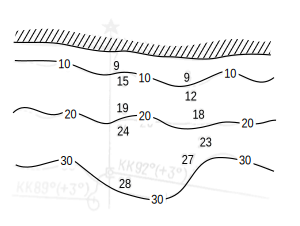
\includegraphics[width=\linewidth]{N051}
  \caption{Опознание места по пеленгу и глубине}
  \label{fig:N51}
\end{figure} 

Опознание места судна по пеленгу и глубине применяют, если с судна
виден только один ориентир, а глубины в районе плавания изменяются
равномерно. Берут компасный пеленг ориентира и одновременно измеряют
глубину эхолотом. Место судна получают на пересечении линии
исправленного пеленга с отрезком изобаты, соответствующей измеренной
глубине. Изобату наносят, ориентируясь на отметки глубин на
карте. Точность опознанного места будет тем выше, чем равномернее и
ближе одна к другой изобаты.

\section{Проработка перехода. Подбор карт, руководств и пособий для плавания}

Проработка перехода является важнейшей частью штурманской подготовки к
рейсу. Её выполняют заблаговременно в порту получения рейсового
задания. Проработка перехода включает в себя подбор карт, руководств и
пособий для плавания, их корректуру, изучение района плавания, в том
числе навигационной, гидрометеорологической и минной обстановки, выбор
пути и выполнение предварительной прокладки.

\textbf{Подбор карт} на переход делает капитан или штурман по разделу
<<Карты>> откорректированного Каталога карт и книг. Со сборного листа
выбирают сборный лист, охватывающий весь район плавания, включая порты
отхода и прихода. Намечают карандашом маршрут перехода от порта отхода
до порта прихода и выписывают номера карт, через рамки которых
проходит маршрут. Со сборного листа генеральных карт подбирают
генеральную карту перехода. Кроме навигационных карт, из Каталога
выбирают номера вспомогательных справочных и специальных карт. Для
захода судна в порты, на рейды и якорные места подбирают планы. По
выписанным номерам отбирают карты из судовой коллекции.

\textbf{Подбор необходимых на переход Руководств и пособий для
  плавания} осуществляется по сборным листам этих изданий, помещённым
в Каталоге карт и книг в разделе <<Книги>>. Если каких-либо карт или
пособий, нужных в данном рейсе, в судовой коллекции не имеется, их
следует получить в БЭРНК (базовые электрорадионавигационные камеры)
морского пароходства. Все подобранные на переход карты и пособия
корректируют на день выхода в море с учётом последних выпусков ИМ
ГУНиО МО (Извещение Мореплавателям Главное Управление навигации и
океанографии министерства обороны), которые дополучают в БЭРНК или
инспекции портового надзора вместе с прогнозом погоды. Отобранные
навигационные карты укладывают в верхние ящики штурманского стола
лицевой стороной вверх в том порядке, в каком ими будут пользоваться в
рейсе. Первым сверху укладывают план порта отхода, затем генеральную
карту на район перехода, путевые карты и, наконец, план порта
прихода. Лоции и дополнения к ним, книги <<Огни и знаки>>, РТСНО,
наставления для плавания, таблицы и другие издания, которые могут
понадобиться в рейсе, хранят на полке у штурманского стола.

\section{Изучение района плавания, выбор пути и предварительная прокладка}

Изучение района плавания необходимо для выбора безопасного и выгодного
пути судна. При этом нужно получить ясное представление об условиях
плавания в районе перехода. Для этого по откорректированным картам и
Руководствам выбирают сведения о таких навигационно\-/географических
особенностях, как рельеф морского дна, характер изменения глубин,
навигационные опасности и их ограждение, узкости, порты\-/убежища и
т.\=,д. По лоции, атласам и специальным картам изучают
гидрометеорологический режим во время перехода: преобладающие ветры,
вероятность туманов, возможность встречи со льдами, характер
течений. При этом учитывают прогноз погоды по району плавания. Изучают
также объявления об опасных от мин районах и фарватерах для плавания в
них, о режимных районах, рекомендованных путях и системах разделения
движения судов, публикуемые в выпуске \No\=,1 ИМ. Устанавливают
порядок и режим работы радиостанций, передающих гидрометеорологические
сообщения, НАВАРЕА, ПРИП и НАВИП.

В результате тщательного изучения района плавания судоводитель
получает необходимые данные для выбора наивыгоднейшего пути на
переходе. Его намечают с учётом рекомендаций для плавания по
оптимальным путям и прокладывают по генеральной карте. По проложенному
маршруту выделяют зоны вероятного понижения видимости, штормов,
появления льда и намечают меры по преодолению этих
явлений. Рассчитывают протяжённость плавания по линии пути и
продолжительность рейса.
 
Следующим этапом проработки перехода является предварительная
прокладка, выполняемая на путевых и частных картах и планах, на
которых будет вестись в рейсе исполнительная прокладка. Курсы судна
должны быть проложены из расчёта обеспечения плавания не менее чем в
течение двух суток. В дальнейшем предварительную прокладку продолжают
на переходе. В процессе предварительной прокладки рекомендуется
произвести подъём путевых и частных карт и планов. Подъём карты
заключается в выделении на ней опасностей, проведении ограждающей
изобаты, нанесении на карту границ секторов огней маяков, их дальности
видимости с учётом своей высоты глаза и т.\=,д. Магнитное склонение по
всему пути судна приводят к году плавания и надписывают карандашом его
значение у меридианов под верхней горизонтальной рамкой. При плавании
вблизи берегов точки поворота на новые курсы следует выбирать по
пеленгам ориентиров. Для районов с приливо\-/отливными явлениями
рекомендуется заранее рассчитывать время наступления полной и малой
вод, смены направлений течений, а также поправки глубин для портов и
якорных стоянок. На каждом участке подбирают ориентиры, обеспечивающие
наиболее надёжное определение места судна.
 
Особое внимание уделяют выполнению предварительной прокладки для
плавания в стеснённых районах и на подходах к портам. В частности, при
прокладке курсов учитывают требования местных правил, лоций,
установленные системы разделения движения, принимают во внимание
поправки на течение. Линии курсов прокладывают на безопасном
расстоянии от препятствий, на них отмечают точки начала и конца
поворотов; проводят линии поворотных пеленгов на выбранные
ориентиры. Там, где линии курсов проходят близко от опасностей, на
карты наносят ограждающие изолинии: дуги опасных расстояний и углов,
линии опасных пеленгов. На линии курсов надписывают их истинные
значения. Измеряют плавание по каждому курсу и по путевой скорости
определяют время следования по ним. С материалами проработки перехода
знакомится весь штурманский состав судна.

\section{Плавание при ограниченной видимости и в стеснённых условиях}

\begin{figure*}[htb]
  \centering{}
  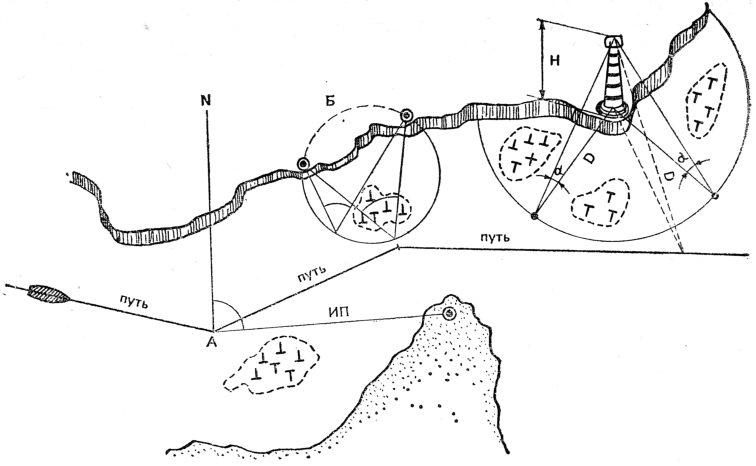
\includegraphics[width=0.8\linewidth]{0086P}
  \caption{Ограждающие (опасные) изолинии}
  \label{fig:N86}
  \small
  \centering{}
  ИП \--- опасный пеленг; $\beta$ \--- горизонтальный угол опасности; $D$ \--- опасное расстояние; $\alpha$ \--- вертикальный угол опасности
\end{figure*}

Малая видимость может возникнуть из-за осадков, пурги, тумана и
составлять от нескольких кабельтовых до 20\otdo 40~м. В тумане
становятся невидимы огни маяков, знаков, судов и другие средства
навигационного обеспечения. Повышается вероятность столкновения с
другими судами. При плавании в мелководном районе возникает опасность
посадки яхты на мель.
 
При первых признаках снижения видимости и появления тумана капитан
яхты должен надёжно определить своё место и при необходимости изменить
курс, чтобы обеспечить безопасное плавание в тумане или стать на якорь
в районе, удалённом от рекомендованных курсов судов. Счисление пути в
тумане должно вестись особенно тщательно, с учётом поправок приборов,
а при необходимости дрейфа и течения. Участие в этом и контроль
капитана яхты обязательны. В отсутствие лага периодически (ежечасно)
измеряют скорость хода, чтобы учитывать её при счислении. Необходимо
постоянно контролировать своё место по GPS и как дополнительный
контроль использовать эхолот, сверяя глубину с таковой на карте. Если
есть радиолокатор \--- держать его включённым, контролируя
пространство вокруг яхты.
 
Кроме того, при плавании в условиях малой видимости включают ходовые
огни, держат у рулевого наготове мощный фонарь, ракетницу с белой
звездой и фальшфейеры, поднимают радиолокационный отражатель, готовят
к отдаче якорь и дают туманные сигналы согласно ППСС. Одновременно
выставляют вперёдсмотрящего для наблюдения и прослушивания туманных
сигналов судов и средств ограждения. На яхте соблюдается тишина. Если
капитан яхты не уверен в безопасности плавания, то необходимо, когда
возможно, отдать якорь и отстояться до уточнения обстановки.
 
К стеснённым условиям относят участки плавания вблизи берегов,
островов, навигационных опасностей. Это могут быть проливы, шхеры,
каналы и другие узкости. При плавании в стеснённых районах пользуются
картами крупных масштабов. Предварительно тщательно изучают район
предстоящего плавания, навигационную обстановку в нем, систему
ограждения (берегового и плавучего), подбирают ведущие и секущие
поворотные створы и места возможных якорных стоянок. Следует помнить,
что в узкостях повышается опасность столкновения, особенно на створах
и фарватерах с активным движением судов и кораблей. При наличии
двигателя такие участки проходят под мотором.

При проходе стеснённых районов местность постоянно сличают с
картой. Яхту ведут по рассчитанному \KK, определяя место как
пеленгованием, так и на глаз при проходе в непосредственной близости
от опознанного плавучего знака. Опознавая имеющиеся на карте ориентиры
\--- острова, мысы, знаки ограждения, замечают время (при наличии \---
и лаг), делают карандашом пометки на карте и в блокноте, одновременно
выбирают с карты ориентиры, которые должны открыться, и ищут их в
соответствующем направлении. Время и место всех поворотов отмечают
карандашом на карте и записывают в блокнот, анализируя расхождение
расчётных и фактических данных. Если есть лаг, сравнивают проходимые
между знаками расстояния по лагу и по карте. По мере необходимости
нужно проверять глубину лотом или эхолотом.

Надо помнить, что слепо полагаться на положение плавучих знаков
нельзя, нужно подстраховывать их контрольными пеленгами, например, при
каждом повороте. Для обеспечения безопасности плавания в узкостях
нередко применяют метод ограничительных (опасных) изолиний. Чаще
применяют ограничительный пеленг. Для этого от хорошо видимого
ориентира проводят на карте линию пеленга, ограничивающую опасность
(рис.~\ris{N86}). При проходе мимо этой опасности следят, чтобы
пеленги на этот ориентир были больше (меньше) ограждающего пеленга.

\section{Судовой журнал и его ведение}

\textbf{Судовой журнал} \--- единственный официальный документ на яхте
в плавании. В нем отражают все навигационные и метеорологические
элементы плавания, внешней обстановки и режима. В походах ведут его
непрерывно с момента прибытия экипажа на яхту перед выходом и до
окончания плавания. В случае гибели судна капитан должен принять меры
к сохранению журнала.
 
На титульном листе журнала (см. рис.~\ris{j-title}) пишут название
яхты, яхт-клуб, порт приписки и даты начала и окончания ведения
журнала. Следующие несколько листов содержат бланки различных
навигационных таблиц и графиков. Среди них: таблицы и график девиации,
таблица определения скорости по базе или способом <<голландского
лага>>, поправки лага, таблица значений углов дрейфа.

\begin{figure}[htb]
  \centering{}
  \fbox{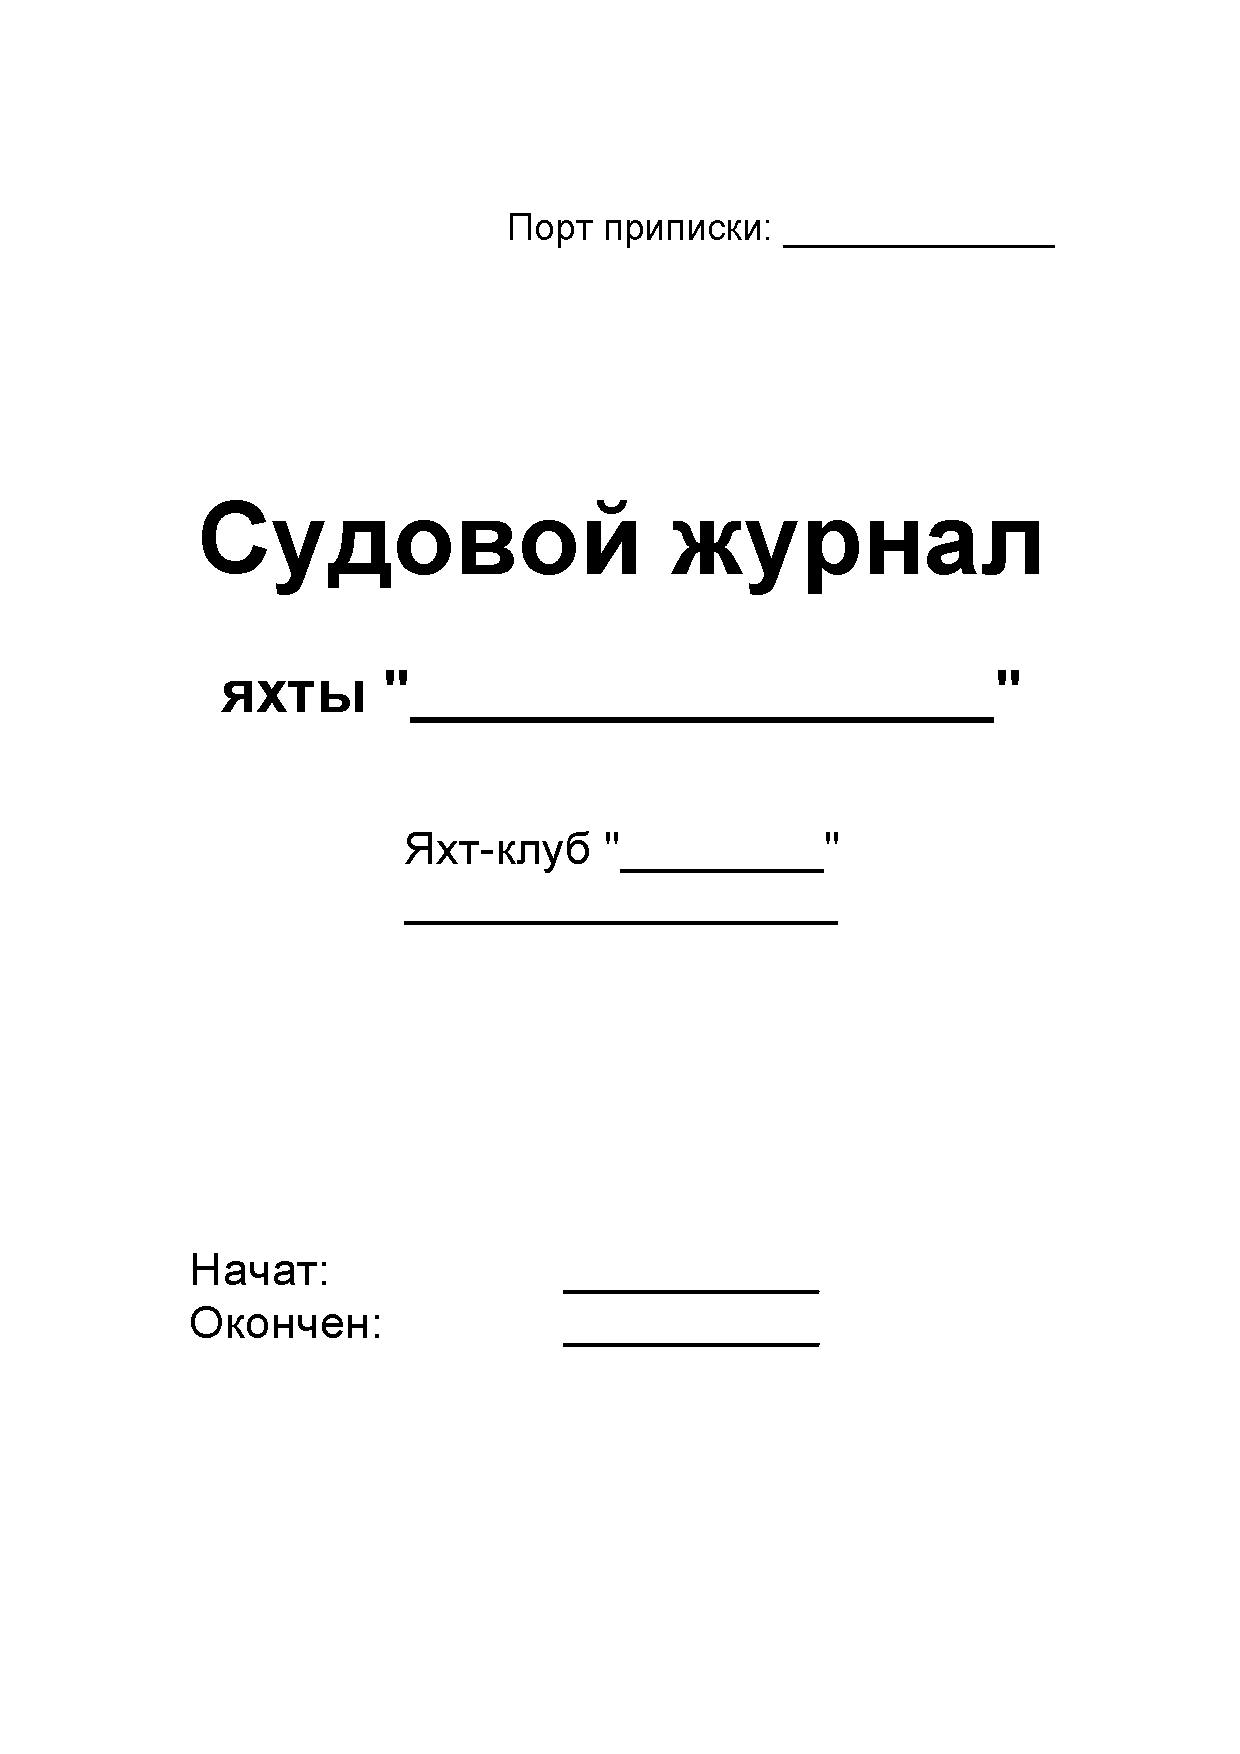
\includegraphics[width=0.8\linewidth]{j_title}}
  \caption{Образец титульной страницы судового журнала}
  \label{fig:j-title}
\end{figure} 

\begin{figure*}
  \begin{minipage}{0.49\textwidth}
    \centering{}
    \fbox{\includegraphics[width=0.8\linewidth]{j_pages_1}}
    \caption{Вторая страница судового журнала с описание правил ведения}
    \label{fig:j-page-1}
  \end{minipage}
  \hfill\hfill
  \begin{minipage}{0.49\textwidth}
    \centering{}
    \fbox{\includegraphics[width=0.8\linewidth]{j_pages_2}}
    \caption{Третья страница судового журнала с описание правил ведения}
    \label{fig:j-page-2}
  \end{minipage}
\end{figure*} 

\begin{figure*}
  \begin{minipage}{0.49\textwidth}
    \centering{}
    \fbox{\includegraphics[width=0.8\linewidth]{j_pages_3}}
    \caption{Левая страница судового журнала}
    \label{fig:j-page-3}
  \end{minipage}
  \hfill\hfill
  \begin{minipage}{0.49\textwidth}
    \centering{}
    \fbox{\includegraphics[width=0.8\linewidth]{j_pages_4}}
    \caption{Правая страница судового журнала}
    \label{fig:j-page-4}
  \end{minipage}
\end{figure*} 

Записи в судовом журнале делает вахтенный начальник \--- он ставит в
нем свои подписи при приём и сдаче вахты. Капитан яхты несёт
ответственность за своевременное и исчерпывающее заполнение всех граф
журнала.
 
С началом плавания на первой странице в верхней строке пишут название
пункта отхода, дату и месяц. Затем время снятия с якоря и швартов,
цель и маршрут плавания состав экипажа с указанием должностей, данные
о ветре, волнении, видимости и поставленных парусах либо о включении
двигателя и эволюциях яхты при выходе из гавани. Далее на той же
правой странице (см. рис.~\ris{j-page-4}) должны идти записи о
прохождении фарватеров и траверзов, вех, буев, знаков с указанием их
названий, расстояний и борта прохождения знаков (правый, левый), а
также следующие сведения:

\begin{itemize}
\item курсы относительно ветра и компасного меридиана и их изменение; 
\item прохождение створов с указанием \KP створа и $\Delta \MK$; 
\item способы обсервации с указанием объектов наблюдений, значение измеренных навигационных параметров и поправок приборов, величина и направление невязки, суждение о ней и решение о принятии в расчёт полученной обсервации; 
\item значение отдельных измеренных навигационных параметров на ориентиры и их название; 
\item работа с парусами (смена, рифление, уборка и т.\=,п.);
\item изменение направления и силы ветра, волнения, видимости; 
\item моменты начала и окончания учёта дрейфа с указанием знака и величины угла $\alpha$; 
\item моменты начала и окончания учёта сноса от течения с указанием направления и величины вектора течения, а также знака и величины угла $\beta$; 
\item результаты измерения скорости хода с указанием способа измерения; 
\item время вхождения в полосу тумана и принятые меры; 
\item подача туманных сигналов; 
\item включение ходовых огней; 
\item судовые работы; 
\item время и место досмотра яхты кораблями погранвойск; 
\item случаи несоответствия навигационного ограждения в районе плавания данным карт и пособий; 
\item касание грунта, посадка на мель и снятие с неё; 
\item аварии, поломки рангоута, частей корпуса, приборов, случаи разрыва парусов, такелажа и утраты имущества; 
\item случаи перехода на другую карту с указанием координат точки перехода; 
\item вход в стеснённый район, гавань, канал; 
\item спуск на воду рабочего тузика и подъём его; 
\item постановка на якорь, глубина и грунт в районе отдачи якоря, длина вытравленного якорного каната, компасные пеленги на береговые ориентиры и т.\=,д. 
\end{itemize}

Все записи на правой странице журнала привязывают ко времени, а если
есть лаг, записи навигационных элементов содержат также отсчёты лага.

Левая страница журнала (см. рис.~\ris{j-page-3}) заполняется в
соответствии с её графами при каждом изменении курса и смене
вахты. При плавании в узкостях в условиях, требующих непрерывного или
частого изменения курса, в графе <<Курс>> пишут <<пер>>
(переменный). При наличии лага его отсчёт пишут в графе <<Лаг>>; если
лага нет, пишут скорость в узлах.

Правая и левая страницы связаны между собой по времени, и если одна из
них заполнена полностью, то на оставшемся свободном месте другой
страницы проставляют <<Z>> и следующие записи продолжают на новых
страницах.

Во время вахты записи часто ведут в черновом блокноте, а затем к сдаче
вахты переносят их в судовой журнал. По окончании каждого перехода
капитан яхты (штурман) записывает на левой странице пройденное за
время перехода расстояние по генеральному курсу и фактическое число
ходовых часов (с учётом лавировки), среднюю скорость по генеральному
курсу и по прокладке.

Все записи в судовом журнале делают аккуратно простым
карандашом. Стирать ошибочные записи запрещается. Ошибки в записях
зачёркивают тонкой линией, заключают в скобки, делают сноску
<<зачёркнуто>>, и ведущий журнал ставит свою подпись.

\section{Если яхта на переходе лишилась приборов}

На сегодняшний день, системы GPS стали доступнее и дешевле секстанов,
не говоря уже об удобстве пользования ими. Подкупает точность прибора,
обилие выдаваемых данных и готовность к работе в любое время суток при
любых метеоусловиях. При этом, штурманская работа обычно сводится к
планированию перехода и, в процессе его, графическому нанесению
определённых прибором точек на карту, для визуального контроля
истинного положения судна относительно линии генерального курса. Такая
практика принята даже на больших коммерческих судах, не говоря уже о
яхтах. При этом на яхтах обычно не утруждают себя определением
девиации \--- ведь при ведении яхты на дисплее GPS всегда отразится
абсолютное значение расхождения курса яхты и путевого угла, и это
значение сразу компенсируется соответствующей командой рулевому.

Однако, чем сложнее система, тем выше вероятность того, что сбои в её
работе окажутся незамеченными. Существенное дестабилизирующее влияние
на работу электронной навигационной аппаратуры оказывают многие
факторы: колебания питающих напряжений, повышенная влажность, грозы,
полярные сияния, магнитные бури, сбои в приёме сигналов из-за
повреждения антенны. В исключительных случаях все приборы, включая
компас, просто могут выйти из строя. И вот к такому повороту событий
судоводитель частенько оказывается психологически не готов.

Итак, в результате уникального сочетания природных катаклизмов и
человеческих ошибок (далее <<ЧП>> \--- чрезвычайного происшествия),
яхта лишилась части (или даже всех) приборов. Что делать?

Основное правило \--- не теряйте спокойствия. Катастрофы не произошло,
всего\-/навсего у вас несколько поубавилось средств ориентации. Но
оставшихся вполне достаточно для безаварийного окончания перехода!

Прежде всего, проанализируйте все данные, которыми вы располагаете, а
именно:

\begin{itemize}
\item исправность курсоуказателя; 
\item текущее местоположение и точность его определения; 
\item расстояние до пункта прибытия и сложность навигационной обстановки по ходу. 
\end{itemize}

\textbf{Курсоуказатель.} По принятым на данный момент нормам снабжения
яхты на борту должно находиться 2 компаса и крайне маловероятно, чтобы
сразу оба вышли из строя. Однако возможность такого события не
исключена. Надо лечь на любой курс, выдерживая его по колдунчикам или
другим удобным для рулевого указателям, и пронаблюдайте за показаниями
компасов (компаса). В результате визуальной проверки вы можете
установить одно из трёх:

\begin{itemize}
\item компасы целы и, судя по идентичности показаний, исправны;
\item работает (судя по стабильности показаний и уверенного
  отслеживания манёвров яхты) один компас, но точность его показаний
  под сомнением;
\item компасы не работают (размагничены, разбиты, утеряны и т.\=,п.).
\end{itemize}

\textbf{Текущее местоположение.} Нанесите на карту последнее
определённое по GPS, либо другим надёжным способом, место. Сделайте
графическую прокладку от неё до точки вашего нахождения на данный
момент. Оцените радиус возможной погрешности и прочертите этим
радиусом круг вашего местоположения.

По карте определите компасный курс и расстояние от вашего
местоположения до пункта назначения. Оцените, насколько опасен в
навигационном отношении путь \--- мели, рифы, затонувшие корабли и
т.\=,п. Посмотрите на карте и по лоции расположение в вашем районе
больших портов и оживлённых морских путей (проходящие суда \--- это
замечательные ориентиры, если знать откуда и куда они направляются).

\textbf{Организуйте приемлемый для вас метод измерения скорости.} Это
может быть самодельный лаг, по типу традиционного секторного, или же
измерения способом <<по базе>> (или же
\textit{<<голландский лаг>>}\index{лаг!голландский}, т.\=,е. за
базу принимается длина яхты и засекается секундомером прохождение
щепки от носа до кормы, результат пересчитывается в узлы). Если
принимается решение сделать \textit{ручной лаг}\index{лаг!ручной} (его точность гораздо выше, чем
у <<голландского>>), то удобно задать расстояние между двумя мерными
марками (т.\=,е. <<базу>> лага) равное 30,88~м. Тогда прохождению
<<базы>> за 60 секунд будет соответствовать скорость в 1 узел, 30
секунд \--- 2 узла и т.д. (см. таблицу):

\begin{tabular}{c|c||c|c}
  \toprule
  Сек & Узлы & Сек & Узлы \\
  \midrule
  60 & 1,0 & 12 & 5,0 \\
  40 & 1,5 & 11 & 5,5 \\
  30 & 2,0 & 10 & 6,0 \\
  25 & 2,5 & 9  & 6,5 \\
  20 & 3,0 & 8  & 7,5 \\
  17 & 3,5 & 7  & 8,5 \\
  15 & 4,0 & 6  & 9,5 \\
  \bottomrule
\end{tabular}

Теперь трезво оцените все собранные данные с точки зрения безопасности
продолжения перехода по прежнему маршруту.

Если компас у вас вне подозрений, на вашем пути нет особых опасностей,
а пункт вашего прихода является оживлённым портом \--- можете смело
продолжать переход по прежнему плану, производя графическую прокладку
на карте.

Если подход к берегу требует точности (обилие навигационных
опасностей, незнакомый пустынный берег и т.\=,д.) и/или компас под
подозрением, то надо продумать шаги для уточнения своего
местоположения по ходу. К примеру, если неподалёку от вашего
генерального курса есть чёткие ориентиры (выступающие в море мысы,
освещённые буровые вышки, маяки и т.\=,д.), вероятно, стоит
отклониться от курса во имя возможности визуальных
обсерваций. Возможно, стоит проложить курс не на конечную цель
перехода, а на ближний к ней хорошо опознаваемый ориентир (порт, мыс,
маяк и т.\=,д.), и уже после надёжного его опознавания идти вдоль
берега в конечный пункт, контролируя место визуальными
определениями. В каждом случае производится скрупулёзный учёт всех
параметров движения и делается графическая прокладка, с учётом
возможного накопления ошибок счисления.

Но если ваш путь изобилует навигационными опасностями, а на яхте нет
даже компаса, то, возможно, есть смысл проложить путь на ближайший
порт с безопасным подходом, а там отремонтировать компас, или же идти
в пункт назначения в каботажном режиме, производя обсервации по
береговым ориентирам.

Средства ориентирования при следовании без компаса: 

\begin{itemize}
\item по небесным светилам \--- солнце, полярная звезда;
\item по проходящим судам \--- если достоверно известно направление их
  движения, исходя из близости крупных портов, стратегических
  проливов, устьев судоходных рек;
\item по направлению на известные широковещательные радиостанции \---
  если точно известно их местонахождение. При этом пользуются
  обыкновенным транзисторным приёмником. Его ферритовая антенна
  обладает направленной диаграммой приёма. Максимум приёма находится
  по перпендикуляру к оси антенны, минимум \--- по оси. Пеленгуют на
  диапазонах СВ или ДВ, после опознания станции <<ловят>> направление
  на неё \textbf{по минимуму слышимости}.
\end{itemize} 

Используйте все эти и любые другие представившиеся возможности для
уточнения курса. И, при этом, сразу <<привязывайте>> нужный вам курс к
направлению ветра и волны. Хороший рулевой может выдерживать курс по
колдунчиках (или по передней шкаторине стакселя) длительное время и с
достаточной точностью, не хуже чем по компасу, особенно на острых
курсах. А стабильность направления ветра контролируйте по волне,
которая инерционна по определению, и внезапно изменить направление
своего движения не может (исключая подход принципиально другой
волновой системы, сформированной в другом районе моря, но это всегда
видно).

Если предстоит чистая лавировка (длительность галсов примерно равна),
то идите по передней шкаторине галсами, которые численно равны по
времени.

В любом случае, спланируйте ваш путь таким образом, чтобы оказаться в
районе повышенного внимания (подход к неосвещённому низкому берегу,
район навигационных опасностей и т.\=,д.) по возможности \textbf{в
  светлое время суток.}

\textbf{Переход.} В любом избранном вами варианте, в простых или
сложных условиях, с компасом или без него, постоянно анализируйте
изменения в окружающей обстановке с целью получить дополнительную
информацию. Вот примеры:

\begin{itemize} 
\item \textbf{Изменение цвета и прозрачности воды.} Чаще всего это
  означает близость устья крупных рек, вода которой отличается от
  морской по цвету и прозрачности. Такой же эффект может наблюдаться
  после шторма вблизи берега с илистым дном. На карте выделите
  возможный район распространение воды реки с учётом местных течений,
  примите во внимание сводки погоды и \--- делайте выводы.
\item \textbf{Появление плавающих предметов, травы, водорослей,
    плавника} также служит одним из признаков близости берега. Обилие
  промышленного мусора частенько свидетельствует о близости порта, в
  частности, с оживлённым движением. И хотя плавающие водоросли и
  различные обломки могут встречаться и в значительном удалении от
  берега (учтите течения!), в условиях ограниченной видимости следует
  считать их признаками непосредственной близости берега.
\item \textbf{Изменение характера волнения моря при сохранении общего
    направления и силы ветра.} Во-первых, с уменьшением глубины волна
  становится более крутой и беспорядочной по внешнему виду, поскольку
  уменьшается длина волны, а высота её растёт. Во-вторых, если ветер с
  берега, то при приближении яхты к нему волна, лишаясь разгона, будет
  уменьшатся. В-третьих, усиление волнения вблизи берегов служит
  признаком того, что с наветренной стороны судна имеется значительный
  разрыв береговой черты \--- залив, лиман, устье крупной
  реки. В-четвёртых, если волна, идущая с моря встречается с течением,
  то крутизна её ощутимо возрастает \--- обычное явление неподалёку от
  устья реки.
\item \textbf{Местные изменения направления ветра}, сопровождающиеся
  его усилением, могут наблюдаться при прохождении судна в
  непосредственной близости от глубоких лощин, ущелий, заливов, при
  входах в узости, около низких перешейков высоких скалистых мысов и
  т.\=,п. Вблизи высокого ровного берега, ветер практически всегда
  ослабнет. Об этом необходимо помнить в туман и ночью!
\item \textbf{Появление в значительном количестве морских птиц и
    зверя.} В хорошую погоду птицы залетают далеко в море, но при
  штормовой погоде они держатся ближе к берегу.
\item \textbf{Шум прибоя} при штилевой погоде может быть слышен на
  значительном расстоянии, особенно при мёртвой зыби. При штормовой
  погоде шум прибоя в большинстве случаев также может быть услышан на
  расстоянии, достаточном для принятия решения. Сама полоса прибоя у
  берегов, выделяясь своей белизной, видна даже в очень тёмную
  ночь. Иногда она может быть замечена судоводителем значительно
  раньше, чем берег, в частности, когда последний низок и окрашен в
  тусклые тона.
\end{itemize}

\section{Штурманское снабжение крейсерских яхт}

Современные крейсерские яхты должны быть снабжены штурманскими
приборами и инструментом, необходимым для навигационного обеспечения
дальних морских плаваний в различных метеорологических условиях. В
комплект штурманского имущества входят:

\begin{itemize}
\item компасы и пеленгаторы; 
\item приборы для измерения скорости в пройденного расстояния; 
\item часы; 
\item секундомеры; 
\item приборы и инструменты для измерения глубины под килем; 
\item секстаны; 
\item приборы спутниковой навигации (GPS); 
\item транзисторный приёмник для приёма сводок погоды и сигналов точного времени; 
\item бинокль; 
\item прокладочный инструмент; 
\item гидрометеоприборы; 
\item пиротехника; 
\item туманный горн. 
\end{itemize}

\section{Магнитный компас, его устройство и установка на яхте}

Магнитные компасы по своему назначению делят на \textbf{главные} и
\textbf{путевые}.

\textbf{Главный компас}\index{главный компас}\index{компас!главный}
является основным
прибором, служащим для непрерывного указания курса и пеленгования в
целях определения своего места в море. Его устанавливают в
диаметральной плоскости яхты, в наиболее открытой части палубы,
обеспечивающей хороший круговой обзор и удобство работы.

\textbf{Путевой компас}\index{путевой компас}\index{компас!путевой}
устанавливают перед рулевым, который ведёт
яхту по заданному курсу.

Основными деталями стандартных 127 и 100 мм магнитных компасов
являются котелок с картушкой, пеленгатор, нактоуз и девиационный
прибор, служащий для компенсации влияния судового железа на его
показания. На яхтах, как правило, компасы устанавливают без нактоузов
и девиационных приборов на пружинных подвесах, закреплённых в латунной
шейке компаса или на кронштейне.

\begin{figure}[htb]
  \centering{}
  \includegraphics[width=\linewidth]{0068P}
  \caption{Разрез котелка магнитного компаса}
  \label{fig:N68}
  \small
  \centering{}
  1 \--- корпус; 2 \--- картушка; 3 \--- поплавок; 4 \--- стрелки; 5 \--- топка; 6 \--- шпилька; 7 \--- курсовые нити; 8 \--- диафрагма; 9 \--- пробка
\end{figure} 

Главной частью котелка (рис.~\ris{N68}) является картушка (2),
магнитная система которой состоит из шести магнитных стрелок (4),
находящихся в латунных пеналах, припаянных к донной части пустотелого
поплавка (3) и расположенных симметрично линии 0\otdo 180\gr
картушки. К поплавку крепится латунный ободок, к которому прикреплён
диск из слюды с наклеенным на него бумажным диском, разделённым на
360\gr. В центре поплавка находится сапфировая или агатовая чашечка
\--- топка (5), опирающаяся на острие шпильки (6), укреплённой в
корпусе котелка. Латунный корпус котелка разделен на две камеры \---
основную (верхнюю) и дополнительную (нижнюю). Дном дополнительной
камеры является латунная диафрагма (8), в которую вставлена
центральная втулка с герметически завинчивающейся пробкой (9). Через
втулку с помощью специальной отвёртки можно заменить шпильку.

Котелок залит раствором спирта, в котором благодаря поплавку,
уменьшающему вес картушки до $4 \pm 0,5$~грамма, трение о шпильку
значительно уменьшается. У внутренних стенок корпуса котелка укреплены
носовая и кормовая курсовые нити (7).

Вертикальная плоскость, проходящая через курсовые нити, является
продольной плоскостью котелка. Эта плоскость должна совпадать с
диаметральной плоскостью яхты. Кроме того, носовая нить является
индексом для отсчёта курса яхты.

К корпусу котелка снизу крепится чашка со свинцовым грузом. В чашке
имеется гнездо для патрона с электрической лампочкой, служащей для
подсветки картушки компаса. Центр тяжести картушки со стрелками
расположен ниже точки опоры, поэтому стрелки всегда находятся в
горизонтальном положении, испытывая полное влияние силы земного
магнетизма.

Сверху котелок герметически закрывается толстым стеклом, которое
прижимается к нему азимутальным кольцом для отсчёта курсовых углов,
имеющим деления от 0 до 360\gr. На любом курсе яхты стрелки и линия
$N-S$ картушки остаются в плоскости компасного меридиана. Котелок
находится в карданном устройстве, обеспечивающем его равновесное
положение, и устанавливается в подвесе так, чтобы 0\gr азимутального
кольца был обращён к носу, а 180\gr \--- к корме.

По окончании навигации котелки магнитных компасов вынимают на зимнее
хранение, контрольную проверку и (в случае необходимости) на
ремонт. При появлении в верхней камере котелка воздушного пузырька
котелок вынимают из пружинного подвеса, переворачивают вверх дном и
плавно покачивают, чтобы пузырёк перешёл в дополнительную камеру. Если
таким образом воздушный пузырёк удалить не удаётся, в котелок доливают
компасную жидкость. При обнаружении застоя картушки необходимо
заменить шпильку. Для этого котелок вынимают из подвеса, ставят вверх
дном, снимают чашку с грузом и вывинчивают пробку диафрагмы. Затем
специальной отвёрткой из комплекта компаса вращением против часовой
стрелки вывинчивают шпильку. Если после замены шпильки застой картушки
сохранится, котелок нужно сдать в ремонт.

На сегодняшний день на яхтах получили распространение компактные
компасы без карданного подвеса. Внутри герметичного прозрачного
корпуса, который посредством фланца крепится к палубе или переборке, в
компасной жидкости плавает подвижная система с картушкой. Подвижная
система отрабатывает крен яхты, заменяя таким образом кардан, а
картушка с магнитными стрелками отслеживает направление магнитного
меридиана. Часто в корпус встроена подсветка. Такие компасы
обеспечивают меньшую устойчивость при качке и разброс показаний при
этом достигает 5 градусов. Но такой же величины достигает на волне
рыскание яхты, поэтому в большей стабильности компаса особого смысла
нет, зато компактность и простота установки с лихвой компенсируют этот
недостаток. Корпус компаса неразборный и в случае разгерметизации
восстановлению не подлежит.

Используются также электронные компасы, которые конструктивно состоят
из блока датчиков, соединённого кабелем с репитером. К основным
преимуществам таких компасов относится удобство считывания информации
рулевым, возможность установки вспомогательного репитера над
штурманским столом и возможность расположения датчиков компаса
максимально далеко от судового железа, минимизируя таким образом
девиацию.

\section{Пеленгаторы}\index{пеленгатор}

Используются для определения пеленгов и курсовых углов. Существуют как
насадки на главный компас и ручные оптические либо электронные.

\begin{figure}[htb]
  \centering{}
  \includegraphics[width=\linewidth]{N0PELENGATOR}
  \caption{Пеленгатор обыкновенный}
  \label{fig:NPELENGATOR}
\end{figure} 

На основании пеленгатора, \textbf{насадки на компас}, установлены
глазная и предметная мишени, а в центре \--- съёмная чашка для
дефлектора (прибора для проведения работ по уничтожению
девиации). Вертикальная плоскость, проходящая через прорезь глазной и
нить предметной мишени и центра пеленгатора, называется визирной
плоскостью. При определении направлений на ориентиры следует помнить,
что снимаемый пеленгатором отсчёт является обратным компасным
пеленгом. При определении курсового угла с использованием пеленгатора
отсчёт снимают с азимутального кольца котелка компаса против индекса
пеленгатора, находящегося слева от глазной мишени. Азимутальное кольцо
и пеленгатор периодически протирают и смазывают вазелином.

\textbf{Ручные оптические пеленгаторы}\index{пеленгатор!оптический}
представляют собой небольшой компас, совмещённый с визирным
устройством и ручкой. Держа прибор за ручку, наводят визир на ориентир
и считывают показания компаса. Такие пеленгаторы чуть менее точны, чем
пеленгаторы\-/насадки, но ими можно пользоваться при любом крене и в
любой точке яхты, таким образом, для них нет <<мёртвых секторов
пеленгования>>.

\textbf{Электронные пеленгаторы}\index{пеленгатор!электронный}
являются по сути усовершенствованными вариантами ручных
оптических. Обычно они имеют память пеленгов, что позволяет
максимально упростить пеленгование: достаточно лишь навести визир на
ориентир и нажать на кнопку. На индикаторе высветится значение
пеленга. Часто пеленгаторы имеют электронную память на несколько
пеленгов, позволяя таким образом в считанные секунды взять пеленги для
обсервации по трём ориентирам.

\section{Измерение скорости и пройденного расстояния}

\index{лаг}Для того чтобы систематически контролировать положение судна и
определять его скорость, на яхтах используют вертушечные
электронно\-/механические и индукционные лаги.

Датчиком лага первого типа служит вращающаяся в набегающем потоке воды
крыльчатка (вертушка), на оси которой закреплён постоянный магнит,
вызывающий периодическое замыкание электрического контакта с частотой,
равной частоте вращения крыльчатки. Шаг крыльчатки рассчитан таким
образом, чтобы она делала заданное число оборотов за одну милю
пройденного расстояния.

Как и всякие приборы, все лаги имеют некоторые погрешности. Поэтому
для получения действительного расстояния, пройденного судном,
необходимо расстояние, измеренное лагом, исправить соответствующей
поправкой. Поправку лага выражают через коэффициент лага \cidx{K}{Л},
который вычисляется с точностью до 0,01 по формуле:
%
\begin{equation}
  \cidx{K}{Л} = \frac{S}{\mcyr{ОЛ}_2 - \mcyr{ОЛ}_1}
\end{equation}
%
где: $S$ \--- действительное расстояние пройденное яхтой,
$\mcyr{ОЛ}_2 - \mcyr{ОЛ}_1$ \--- разница отсчётов лага на этом
расстоянии.

\begin{figure}[htb]
  \centering{}
  \includegraphics[width=\linewidth]{0069P}
  \caption{Секторный лаг}
  \label{fig:N069}
\end{figure} 

При отсутствии на яхте лага определить её скорость можно, одновременно
измеряя время и расстояние (базу). Для этого нужно изготовить прибор в
виде секторного лага (рис.~\ris{N069}), но вместо узлов на лаглине
вплести только одну цветную марку на расстоянии 20 м от сектора. Для
того чтобы измерить скорость, сектор опускают за борт и при
прохождении кормового среза пускают секундомер. Останавливают
секундомер, когда через этот же срез пройдёт цветная марка. Скорость
яхты на галсе вычисляется по формуле:
%
\begin{equation}
  v = \frac{S}{t}\, ,\  \text{м/с}
\end{equation}
%
$S$ \--- длина базы в метрах, $t$ \--- время прохождения базы в
секундах. Если $S = 20$\tmin, тогда приближённо: $v = 40 / t$, узлы.

По этой формуле на каждой яхте должна быть рассчитана таблица или
номограмма для определения скорости судна по известной базе.

Аргументом для входа в таблицу (номограмму) является время $t$
прохождения базы в секундах. Вместо такого прибора можно использовать
заполненную до половины бутылку с лаглинем, закреплённым на горлышке.

Иногда измеряют скорость с помощью так называемого
\textbf{голландского лага}\index{лаг!голландский}.  В этом случае
базой является длина яхты, а для измерения времени $t$ секундомер
запускают и останавливают при прохождении форштевня и кормы мимо
сброшенного на воду небольшого предмета (чурки и т.\=,п.). В целях
уменьшения случайных ошибок измерение обычно повторяют несколько раз
(не менее трёх). Вычисление производят аналогично по формуле,
предварительно измерив длину яхты и рассчитав проходимую за время $t$
базу $S$.

При плавании в видимости береговых ориентиров скорость яхты измеряют
по навигационным обсервациям и вычисляют по формуле. При недостатке
ориентиров для обсерваций с достаточной точностью оценивают скорость
яхты при плавании на одном курсе между траверзами двух ориентиров,
нанесённых на карту.

\section{Приборы для измерения глубины}

\index{эхолот}Работа эхолота основана на пьезоэлектрическом
эффекте. Эхолот имеет вибратор\-/излучатель и
вибратор\-/приёмник. Первый излучает под водой механические колебания
в виде коротких ультразвуковых импульсов, которые доходят до дна,
отражаются от него и принимаются вибратором\-/приёмником. По
известному промежутку времени между посылкой и приёмом отражённого от
дна импульса и скорости распространения звука в воде автоматически
вычисляется и указывается на шкале эхолота глубина под килем. Многие
эхолоты имеют самописцы, ведущие запись глубины во времени.

\index{лот ручной}Ручной лот применяют для измерения малых глубин при
скорости хода до 5 узлов или при стоянке на якоре для определения
дрейфа. Он позволяет определить характер грунта. Ручной лот
(см. рис.~\ris{N070}) состоит из свинцовой или чугунной гири (3\otdo
4~кг) и пенькового бельного линя (диаметром 1~мм) кабельной работы
\--- лотлиня, на котором гиря опускается в воду. Гиря в виде конуса
или пирамиды (высотой 15\otdo 20~см и диаметром у основания 5\otdo
7~см) имеет вверху проушину, в которую продевается обшитая кожей
стропка из стального троса. В неё ввязывается огон лотлиня. В
основании гири имеется лунка с поперечным сечением в виде ласточкина
хвоста, куда вмазывается смесь сала с толчёным мелом, к которой
пристают частицы грунта. Длина лотлиня \--- 25~м.

\begin{figure}[htb]
  \centering{}
  \includegraphics[width=\linewidth]{0070P}
  \caption{Ручной лот}
  \label{fig:N070}
\end{figure} 

При плавании в районах с глубинами менее 4 м для определения глубины
на яхтах часто пользуются \textbf{футштоком}\index{футшток}.

\section{Спутниковые системы навигации (GPS)}

Спутниковые навигационные системы включают три элемента: космический
(навигационные ИСЗ), наземный (комплекс управления спутниками) и
оборудование пользователей. Технической основой СРНС и источником
навигационной информации являются 24 ИСЗ, вращающиеся на высоте 20000
км с периодом обращения 12 час и равномерно <<покрывающие>> всю земную
поверхность. Спутники GPS способны, передвигаясь заполнять бреши в
системе (если один из них вышел из строя).

\textbf{Принцип действия.} Сигналы спутника содержат два вида
информации: <<навигационные сообщения>> и <<псевдослучайный код>>. Код
представляет собой последовательность единиц и нулей, на первый взгляд
случайную, но изменяющуюся по сложному закону, индивидуальному для
каждого спутника (рис.\ris{S1}).

\begin{figure*}[htb]
  \centering{}
  \includegraphics[width=0.8\linewidth]{S001}
  \caption[Псевдослучайный код]{Псевдослучайный код (двоичный, состоящий из 0 и 1)}
  \label{fig:S1}
\end{figure*}

Генерация <<псевдослучайного кода>> привязана к шкале времени ИСЗ,
точность которой обеспечена высокоточными атомными часами (рубидиевые
и цезиевые, по четыре на каждом спутнике). <<Навигационные сообщения>>
\--- это данные об исправности спутника и параметры его орбиты
(эфемериды) \--- коэффициенты, которые регулярно уточняются в
результате взаимодействия с наземным комплексом управления спутниками.

Приёмник GPS также содержит генератор, который может повторить
<<псевдослучайный код>> любого из спутников. Работа генератора
привязана к кварцевым часам приёмника.

Итак, на приёмник поступают сигналы со спутника. Дешифровывая эти
сигналы, приёмник идентифицирует его номер и по эфемеридам вычисляет
текущее и будущее положение данного спутника, используя математическую
Кеплеровскую модель. В это же время в приёмнике запускается генератор
кода, точно повторяющего код спутника. При сопоставлении своего кода с
кодом, принимаемым от спутника, определяется суммарный временной
сдвиг, состоящий из двух слагаемых: задержки времени, пропорциональной
дальности до спутника и набегающей погрешности хода кварцевых часов
приёмника.
 
Приёмник GPS имеет программу, которая производит вычисления
основываясь на трёх линиях положения (т.\=,е. по данным, полученным от
трёх спутников). Математически это решение трёх уравнений для трёх
неизвестных: долготы, широты и ошибки часов.
 
В итоге, для определения двухмерных координат приёмнику необходимы как
минимум три спутника, для трёхмерных \-- четыре.

\textbf{Точность.} GPS приёмник при нормальных условиях эксплуатации
обеспечивает точность порядка 15 метров. Скорость индицируется с
точностью не хуже 0,12 узла\footnote{примечание: минимальная скорость,
  при которой прибор индицирует её значение - 2 узла}.

\textbf{ВНИМАНИЕ!} Министерство Обороны США, в чьём подчинении
находится отдел технического обслуживания спутников системы GPS, может
ввести в действие режим селективного доступа к данным, при этом
точность определения для обычных пользователей падает до 100 метров и
более.

Следует также иметь в виду, что приведённую выше точность прибор
обеспечит лишь в том случае, когда между его антенной и спутниками нет
источников помех и поблизости нет источников отражённых сигналов. На
яхте такими источниками обычно являются троса стоячего такелажа. Чтобы
избежать помех необходимо антенну приёмника вынести на топ мачты, либо
на стойку, укреплённую на релинге.

По этим же причинам не стоит размещать антенну прибора непосредственно
около металлических предметов и наклеивать на неё наклейки. Если на
яхте используется ручной прибор, и нет возможности вынести его
антенну, то при определении места следует учитывать возможность ошибки
порядка 150 метров.

Ещё одно требование: расстояние антенны GPS от антенны морского
передатчика мощностью 25 Ватт должно быть не меньше 1 метра.

\textbf{Координатные системы карт (Map Datum).} По историческим
причинам геодезические департаменты разных стран используют различные
модели земного шара. Карты, составленные по разным моделям, дают разные
координаты одного и то-же места. Эта разница может достигать 500
метров.

В память приёмника GPS обычно занесено несколько координатных системах
(Map Datum). По умолчанию установлена WGS84 (ещё есть WGS72, OSGB36,
NAD27 и другие). Если одна из этих систем соответствует координатной
системе Вашей навигационной карты, то следует её активировать.

Если координатная система Вашей карты неизвестна, то лучше
пользоваться WGS84. При каждом удобном случае сравнивайте координаты
надёжного ориентира, отмеченного на карте с координатами,
определёнными в этой же точке приёмником GPS. Направление и величина
невязки записываются в вахтенный журнал и учитываются при работе с
GPS.

\textbf{Первичная инициализация.} Для определения координат прибор
нуждается в знании текущей даты, времени и примерного местоположения
на Земном шаре с точностью до 300~км. Поэтому при первом включении,
либо после длительного хранения без батарей, прибор нужно
инициализировать (см. инструкцию).

\textbf{Работа прибора.} После включения GPS находит своё
местоположение и начинает периодически его сканировать, отслеживая
изменение координат, вычисляя при этом скорость $V$ и курс яхты \IK
(или \MK, см. инструкцию).

В каждом современном приёмнике GPS есть функция запоминания
координат. При этом позиция записывается под выбранным пользователем
именем в библиотеку путевых точек (в разных моделях GPS обозначаемых
как <<WPT>> или <<LMK>>). Записать можно как текущие координаты, так и
любые введённые по данным с навигационной карты. Если после этого
инициировать функцию достижения предварительно введённой путевой
точки, то прибор начнёт непрерывно индицировать дополнительные данные
относительно неё, а именно:

\begin{itemize}
\item истинный или магнитный пеленг на путевую точку \IP (\MP);
\item оставшееся до точки расстояние $D$; 
\item расчётное время достижения точки (при условии неизменности
  скорости) TTG.
\end{itemize} 

Ещё больше информации выдаст прибор при активации маршрута. Каждый
приёмник GPS имеет память на как минимум один маршрут, который штурман
заранее вводит в память, путём указания запрограммированных путевых
точек в последовательности соответствующей предварительной прокладке
предполагаемого пути. При активации выполнения маршрута прибор,
сравнивая текущее место яхты с заданной линией пути по предварительной
прокладке, кроме всего вышеперечисленного выдаёт также текущее
расстояние яхты от заданной линии пути XTE и направление и величину
коррекции курса для выхода на эту линию пути.

\section{Задачи, решаемые при помощи GPS}

\begin{figure*}[htb]
  \centering{}
  \includegraphics[width=0.8\linewidth]{S002}
  \caption{Коррекция курса яхты с использованием GPS}
  \label{fig:S2}
\end{figure*}

\begin{figure*}[htb]
  \centering{}
  \includegraphics[width=0.8\linewidth]{S003}
  \caption{Контроль счисления пути с использованием GPS}
  \label{fig:S3}
\end{figure*}
 
\begin{figure*}[htb]
  \centering{}
  \includegraphics[width=0.8\linewidth]{S004}
  \caption{Контроль перехода в заданную точку с использованием GPS}
  \label{fig:S4}
\end{figure*}

\begin{figure*}[htb]
  \centering{}
  \includegraphics[width=0.8\linewidth]{S005}
  \caption{Предварительная прокладка с использованием GPS}
  \label{fig:S5}
\end{figure*}

\textbf{Коррекция курса яхты.} Во время следования по линии
генерального курса в точку назначения, периодически определяют
местоположение при помощи GPS и наносят на карту. Если полученная
таким образом линия пути отличается от линии истинного курса на
какой-то угол, то этот угол вычитают из компасного курса. Продолжают
путь по откорректированному значению \KK, продолжая периодически
контролировать местоположение (см. рис.~\ris{S2}):

\textbf{Контроль счисления пути.} Штурман яхты, проложив на карте
линию пути с учётом склонения, дрейфа и течения, имеет возможность в
любое время снять координаты с дисплея GPS и нанести их на карту. Если
полученная точка совпадает со счислимой, или расходится с ней
незначительно, \--- счисление пути судна ведётся правильно. Если нет
\--- в счисление вносят поправку (аналогично предыдущему пункту).

\textbf{Пример.} В момент $T_0$ начато счисление пути яхты для
следования путевым углом $\PU = 108,5\gr$ при склонении 1,5\gr\,Е на
курсе $\KK = 110\gr$ без учёта сноса (см. рис.~\ris{S3}). В ходе
плавания счисление контролировалось по GPS, координаты точек, снятые с
дисплея в $T_1$, $T_2$, $T_3$ нанесены на карту. Последнюю обсервацию
приняли для дальнейшего счисления. Выявлено, что фактический путевой
угол яхты на 25\gr больше расчётного, для сохранения заданного
путевого угла изменили курс на 25\gr влево. Продолжили счисление с
учётом суммарного сноса, продолжая периодический контроль.

\textbf{Контроль перехода в заданную точку по GPS.} С карты снимают
координаты точки назначения и заносят в память GPS (LMK1). На карте
выбирают также <<коридор безопасности>> \--- величина допустимого
отклонения яхты в обе стороны от оси движения без риска входа в зону
опасности (с учётом погрешности от разности в Map Datum). Прибор
индицирует такое отклонение как параметр XTE (см. рис.~\ris{S4}).

В начале перехода активируется функция (обычно функция "GO TO")
достижении точки LMK1. Яхту ведут по компасу, регулярно контролируя
величину XTE. Если она имеет постоянную тенденцию к увеличению, то в
\KK вносят компенсирующую поправку.

\textbf{Предварительная прокладка.} Возможность программирования
маршрута предстоящего перехода путём введения в память прибора путевых
точек (LMK) и очерёдности их достижения очень упрощает работу штурмана
на маршруте и снижает риск возможных ошибок при счислении и прокладке
пути в дискомфортных условиях и в состоянии усталости, которые столь
характерны при длительном бурном переходе на яхте.

На карту наносят точки выхода и прихода. Отмечают все имеющиеся по
пути следования опасности (<<поднимают карту>>).  Затем выбирается
<<коридор безопасности>> маршрута (предельный XTE). При этом
руководствуются такими данными:

\begin{itemize}
\item наличие узких проходов между опасностями;
\item <<степень доверия>> к карте (год выпуска с учётом коррекций,
  масштаб) и величину возможной невязки по разности Map Datum;
\item вероятность лавировки. 
\end{itemize}

Возможно, на разных галсах маршрута имеет смысл назначить разную
величину XTE.

После этого на карту наносят промежуточные точки маршрута (точки
поворота) с учётом выбранного XTE и дополнительного запаса (расстояние
от опасности до ближайшей границы <<коридора
безопасности>>). Определяют \KK для каждого галса.

Далее все точки маршрута заносят в память GPS-приёмника. 

\textbf{Движение по маршруту.} В начале перехода активируется
выполнение маршрута. На каждом галсе маршрута правят по компасу (\KK
для данного галса), регулярно контролируя величину XTE. Если она имеет
постоянную тенденцию к увеличению, то в \KK вносят компенсирующую
поправку.

В точках поворота прибор сам переключится на отслеживание очередного
галса маршрута.

На лавировке рулевой ведёт яхту по вымпельному ветру, контролируя
изменение величины XTE. При достижении выбранного предельного значения
делают поворот оверштаг и вновь идут отслеживая XTE.

Таким образом, на переходе штурман может быть уверен, что если яхта
отклоняется от оси маршрута не более чем на величину XTE, то она
гарантировано находится вне опасности.

\textbf{Раскладка галсов на лавировке.} Если яхте предстоит лавировка
в открытом море при периодически изменяющемся по направлению ветре, то
активируют функцию достижения заданной путевой точки и закладывают
галсы исходя из разницы истинного курса и истинного пеленга на точку
прихода. Яхту ведут круто к ветру по передней шкаторине стакселя. Если
при этом на галсе индицируемая на приёмнике GPS разница
$\IP - \IK < 45\gr$, то этот галс выгоден, если же нет, то выгоднее
его сменить.

Ещё проще использовать в такой ситуации значение функции VMG
(абсолютная скорость продвижения по генеральному курсу), идя тем
галсом, на котором этот показатель больше (данная функция реализована
не во всех моделях GPS).

В заключение хочется привести цитату из <<Руководства по
эксплуатации>>:

\begin{quote}
  \it Все навигационное оборудование производится и продаётся лишь как
  средство помощи в навигации. Пользователь сам ответственен за
  совершенствование своего навигационного мастерства, независимо от
  любого, приобретённого им оборудования.
\end{quote}

\onecolumn

%%% Local Variables:
%%% mode: latex
%%% TeX-master: "yacht-captain"
%%% End:
